%!TEX encoding = UTF-8 Unicode
%!TEX program = xelatex

\documentclass[bachelor]{ustcthesis}
% bachelor|master|doctor
\usepackage{ustcextra}
\graphicspath{{figures/}}
\bibliographystyle{ustcauthoryear}
% \bibliographystyle{ustcnumerical}

\renewpagestyle{front}[\zihao{-5}]{
    \sethead{}{软件工程作业管理系统概要设计}{}
    \setfoot{}{\thepage}{}
    \headrule
}
\renewpagestyle{main}[\zihao{-5}]{
    \sethead{}{软件工程作业管理系统概要设计}{}
    \setfoot{}{\thepage}{}
    \headrule
}
\newcommand{\HRule}{\rule{\linewidth}{0.5mm}}
\newcommand{\tabincell}[2]{\begin{tabular}{@{}#1@{}}#2\end{tabular}}

\begin{document}



\begin{titlepage}
\begin{center}
~\\[5cm]
\HRule \\[0.4cm]
{\huge \bfseries 软件工程作业管理系统\\概要设计}\\[0.4cm]
\HRule \\[1.5cm]

\begin{tabular}{ccc}
  & 人员 & 日期 \\ 
拟制 & 张三\ 李四\ 王五 & yyyy-mm-dd \\ 
评审人 & • & yyyy-mm-dd \\ 
批准 & • & yyyy-mm-dd \\ 
签发 & • & yyyy-mm-dd \\ 
\end{tabular} 

\end{center}
\end{titlepage}



\frontmatter
\begin{abstract}
本文是软件工程需求规格说明书模板,修改自于中国科学技术大学本硕博毕业论文 \LaTeX{} 模板示例文件,该模板由
zepinglee和seisman创建,遵循中国科学技术大学的论文写作规范,适用于撰写学士、硕士和博士学位论文。

本文档最后一章演示如何使用 \LaTeX{} 的一些基本命令以及本模板提供的一些特殊功能,
模板的选项及详细用法请参考模板说明文档 ustcthesis.pdf。请在提交之前把最后一掌实例注释掉。

\keywords{软件工程\zhspace{} 中国科学技术大学\zhspace{} 学位论文\zhspace{} \LaTeX{}~通用模板\zhspace{} 学士\zhspace{}
硕士\zhspace{} 博士\zhspace{} 示例文档\zhspace{} 模板说明文档}

\begin{table}[htbp]
\centering
\caption{缩略词清单} \label{tab:abbr}
\begin{tabular}{|c|c|c|}
    \hline
    缩略语 & 英文全名 & 中文解释 \\
    \hline
    c & d & e\\
    \hline
\end{tabular}
\end{table}

\end{abstract}

\tableofcontents
\listoffigures
\listoftables
% \listofalgorithms  % 算法索引,如不需要,可直接注释掉本行
% \begin{notation}

%\centering
%XX 软件需求规格说明书

%关键词:能够体现文档描述内容主要方面的词汇。
 
%摘要:


\centering
\begin{tabular}{rl}
$\ln x$ & natural logarithm $\log_ex$ \\
$\log x$ & common logarithm $\log_{10}x$ \\
$x\ \mathrm{mod}\ y$ & remainder \\
\end{tabular}

\end{notation}


\mainmatter
\chapter{引言}
\section{编写目的}
在本项目的前一阶段,也就是需求分析阶段,已经将系统用户对本系统的需求做了详细的阐述,这些用户需求已经在上一阶段中对不同用户所提出的不同功能,实现的各种效果做了调研工作,并在需求规格说明书中得到详尽得叙述及阐明。

本阶段已在系统的需求分析的基础上,对即时聊天工具做概要设计。主要解决了实现该系统需求的程序模块设计问题。包括如何把该系统划分成若干个模块、决定各个模块之间的接口、模块之间传递的信息,以及数据结构、模块结构的设计等。在以下的概要设计报告中将对在本阶段中对系统所做的所有概要设计进行详细的说明,在设计过程中起到了提纲挈领的作用。

在下一阶段的详细设计中,程序设计员可参考此概要设计报告,在概要设计即时聊天工具所做的模块结构设计的基础上,对系统进行详细设计。在以后的软件测试以及软件维护阶段也可参考此说明书,以便于了解在概要设计过程中所完成的各模块设计结构,或在修改时找出在本阶段设计的不足或错误。


\section{项目背景}
随着xxx的不断发展...

\section{术语}
[列出本文档中所用到的专门术语的定义和外文缩写的原词组]
\begin{table}[htbp]
\centering
\caption{术语表} \label{tab:terminology}
\begin{tabular}{|c|c|}
    \hline
    缩写、术语 & 解释 \\
    \hline
    c & d \\
    \hline
\end{tabular}
% \note{这里是表的注释}
\end{table}
\chapter{总体概述}

Describes the general elements that may affect the product and the requirements on the product. It includes the following four parts. Note that this section should not describe the specific requirements, instead, it makes the specific requirements to be described more understandable.

本节描述影响产品和产品需求的一般因素。由以下4个部分构成。 有一点需说明的是本节不描述具体的需求,只是使那些将要描述的具体需求更易于理解。
\section{软件概述}
\subsection{项目介绍}
Describe the context and origin of the project being specified in this SRS. For example, state whether this project is a follow-on member of a project family, a replacement for certain existing systems, or a new, self-contained project.

描述本软件需求所描述的项目的背景。例如:本项目是一系列版本中的一个,或者是替代某个已经存在的系统,还是一个新的独立的项目。

\subsection{产品环境介绍}
Describes the whole environment that is composed of this software and other products / projects.
\begin{itemize}
\item If this software is independent or fully self-contained, state it here.
\begin{itemize}
\item describe the function of each component of that larger system/project, and identify the interfaces.
\item determine the main external interfaces of this software.( Note: Do not describe the interfaces in detail; the detailed description will be provided in other part of the SRS document.)
\item describe related hardware of the product and peripheral equipment.( Note: This is only  a general description, not in detail.)
\end{itemize}
\end{itemize}

It is very helpful to describe the main components, interconnection and external interfaces of the larger system/project by Block Diagram. This part should not provide a detailed design solution, or detailed design constraint for the solution (the detailed design constraint will be described in the section of specific requirement). This section is the basis of the design constraints.

描述的是本产品与其它产品或项目所组成的整体环境。

1.如果本产品是独立的并完全自我包含,在此说明这一点。

2.如果SRS定义的产品是更大的系统或项目的组件(此种情形经常发生),那么应:

	A. 描述此大系统或项目每个组件的功能,并且标识接口。

	B.  确定本软件产品主要外部接口。( 注意:在此部分并不进行这些接口的详细描述;对这些接口的详细描述在SRS的其它 部分提供。)
    
    C. 描述相关产品硬件和所使用的外部设备。(  注意:  这只是概述性描述。)

通过方块图来描述大系统或项目的主要组件,互连性以及外部接口将是非常有帮助的。本部分不应提出一个具体的设计解决方案或对解决方案的具体设计约束(具体设计约束将在具体需求章节中描述)。本部分内容是产生设计约束的基础。

\section{软件功能}
Summarizes the major functions that must be implemented through the software, and the functions to be implemented through user operation. Details will be provided in the Specific Requirement, so only a summary (such as a directory list) is needed here. The functions should be organized to make them understandable to the readers, and be appropriate for subsequent design and tests. Diagrams like top-level data flow diagram or object class diagram are recommended to illustrate the relationships among the major requirement groups 

Sometimes, this section can directly refer to the superior specification of the software that allocate the specific requirements to this software ( if existed ).
The specific requirements should not be described in this section. But this section is the basis of the specific requirements.

概述软件的必须实现的和通过用户操作实现的主要功能。这里只需要进行简要描述(例如目录列表),详细描述在详细需求部分描述。对需求功能进行组织,以便于读者理解,并能指导后续的设计和测试。可以用图表来表示主要需求群组之间的关系,例如:高层的数据流图,面向对象的分析等。

有时此部分所要求的功能概述可以从分配具体功能给此软件产品的更高层规格(如果存在的话)直接引用。

本节不应描述具体需求。但本节内容是具体需求章节的基础。

\section{用户特征}
List down the basic required characteristics of the user or operator of the system. E.g. the experience, Skill level, required role etc., 
This part should not describe the specific requirements, instead, it provides the basis for the specific requirements.

列出对用户或系统操作者的要求,如:经验,能力,角色等。

本节不应描述具体需求。但本节内容是具体需求章节的基础。

\section{假设和依赖关系}
List any assumed factors (as opposed to known facts) that could affect the requirements stated in the SRS. These could include third party or commercial components that you plan to use, issues around the development or operating environment, or constraints. The project could be affected if these assumptions are incorrect, are not shared, or change. Also identify any dependencies the project has on external factors, such as software components that you intend to reuse from another project, unless they are already documented elsewhere (for example, in the vision and scope document or the project plan). 

列出可能影响SRS中需求的所有的假设因素(与已知事实相对而言),包括准备使用的第三方或商业组件,操作和开发环境的问题约束等。如果上述假设不正确、没有被告知或者改变了都将对项目产生影响。列出项目对外部条件的依赖,例如重用其他项目的模块等。如果在其他文档(例如项目计划或范围文档等)里已经描述了,在这里可以不用描述。

\chapter{总体设计}
\section{软件描述}
系统包括前台和后台两个部分。

\subsection{前台}
前台主要功能是:
\subsubsection{学生端}
学生用户需要是相应课程的注册用户,具体需要经过相应老师和教学管理人员的同意,成为相应资源的使用者和课程参与者,同时可参与讨论与资源分享。

\subsubsection{教师端}
教师身份经过认证,教师可以注册生成相应的课程,使用软件辅助教学,进行资源分享和作业等的布置等等。

\subsection{后台}
后台主要功能是:
创建维护用户数据库,存储用户上传的课件作业等信息,对用户的各种请求做出响应。

\begin{longtable}{| c | c | p{7cm} |}
% 首页表头
\caption[]{主要功能} \label{tab:longtable} \\
\toprule[1.5pt]
编号  & 功能 & 简介\\
\midrule[1pt]
\endfirsthead
% 续页表头
\caption[]{主要功能(续)} \\
\toprule[1.5pt]
编号  & 功能 & 简介 \\
\midrule[1pt]
\endhead
% 首页表尾
\hline
\multicolumn{3}{r}{\small 续下页}
\endfoot
% 续页表尾
\bottomrule[1.5pt]
\endlastfoot

R.FUNC.BB.001   &   用户登陆   &   用户在IOS、Android、Web Browse输入账号和密码登录对应账户。登录成功后自动与服务器同步用户数据。   \\
R.FUNC.BB.002   &   作业/实验查询   &   作业/实验查询用于查询作业/实验情况。学生可以查到本人相关课程的作业情况。教师可以查询相应班级所有学生每次作业的提交情况。教学管理人员可以查询到自己所负责所有学生相应的作业提交情况。   \\
R.FUNC.BB.003   &   作业/实验/通知发布   &   作业/实验/通知发布仅供教师端和管理人员使用。可以用于教师发布自己负责课程相关的作业、实验或通知。\\
R.FUNC.BB.004   &   作业/实验/通知修改删除   &   仅供教师和管理人员使用。用于修改或删除已发布的作业/实验/通知  \\
R.FUNC.BB.005   &   作业/实验/通知提交   &   仅供学生使用。学生提交完成的作业、实验或需要提交材料的通知。   \\
R.FUNC.BB.006   &   作业/实验查看与批改   &    仅供教师端使用。作业/实验查看与批改用与教师查看学生相应的作业或实验。   \\
R.FUNC.BB.007   &   成绩录入   &   成绩输入仅供教师端使用。可以用于登记考试/作业等等的成绩。   \\
R.FUNC.BB.008   &   成绩查询   &   成绩查询用于查询已经录入的成绩。学生可以查到本人相应课程的所有成绩。老师可以查到相应班级所有同学的成绩。教学管理人员可以查询自己所负责所有学生的相应成绩。   \\
R.FUNC.BB.009   &   成绩统计和调整   &   成绩统计功能教学管理人员与老师都拥有,成绩调整只有老师有相应的权限。成绩统计可用于老师和教学管理人员了解教学情况以及学生的学业状况。成绩调整可以供老师修订成绩同时也可以方便按照一定的规则对于成绩进行统一调整使得成绩更有一般性并能更好的体现学生的水平。  \\
R.FUNC.BB.010   &   资源上传   &   资源上传可用于教师分享课件等教学辅助材料。同时同学自身也可以分享有用材料。空间分为共享和私有两部分。私有空间可以用作个人文件的托管和同步。  \\
R.FUNC.BB.012   &   资源下载与浏览   &   资源下载用于获取远端分享的相关资源   \\
R.FUNC.BB.013   &   新建日程   &   本功能用于生成新的日程安排,辅助用户合理安排各项任务   \\
R.FUNC.BB.014   &   日程显示与提醒   &   日程提醒显示用于提醒自身的任务安排,合理安排时间。避免遗忘重要事项。   \\
R.FUNC.BB.015   &   讨论区讨论   &   讨论区可以发布新的主题用于进行问题讨论,增强对知识的理解和应用,可在讨论区中发布新主题,修订,回复。   \\
R.FUNC.BB.016   &   新建博文   &   博文主要用于用户分享学习经验等等认为有意义的东西,相比讨论区更加系统。   \\
R.FUNC.BB.017   &   课程考试排布   &   课程考试排布功能主要用于辅助教学管理人员合理安排相关活动,减少冲突节约时间。   \\
R.FUNC.BB.018   &   学习笔记文本添加   &    学生用户在课堂或者课下记录笔记,选择创建新的笔记或者修改已经存在的笔记,进入文本编辑界面进行,编辑完成后点击保存到本地或者上传,点击返回键退出。   \\
R.FUNC.BB.019   &   学习笔记课件修改   &   学生用户在老师上传的课件上使用文本框或者画图功能添加批注笔记。   \\
R.FUNC.BB.020   &   学习笔记搜索   &   对笔记(文本模块和课件模块)进行检索,可根据创建时间,修改时间,课程,文本进行搜索。   \\
R.FUNC.BB.021   &   学习笔记删除   &   删除某一笔记   \\
R.FUNC.BB.023   &   学习笔记共享   &   用户与其他用户共享学习笔记。 \\

\end{longtable}


\section{处理流程}
\subsection{总体流程}
此处应当有一个图和对应的描述。

\subsection{系统基本流程}
此处应当有一个图和对应的描述。

\subsection{客户端基本流程}
这只是举个例子,如果没有客户端则不需要此节。

\subsection{服务器端基本流程}
这只是举个例子,如果没有服务器端则不需要此节。

\subsection{R.FUNC.BB.001   用户登陆}
客户端发送查询请求到服务器用户数据库,匹配该用户邮箱或学号和密码,匹配成功则返回成功登录的信息,并同步数据,进入登录后页面。匹配失败则返回失败信息,并显示账户不存在或密码错误。若为新用户,客户端发送新建请求到服务器数据库,检查是否为新用户,若可创建则返回允许创建信息,失败则返回无法创建新用户。

\subsection{R.FUNC.BB.002   作业/实验查询}
已登录用户在作业实验模块中提交查询请求,提交的表单中指明查找的关键字,由客户端和服务器端从本地存储和服务器存储的的数据文件进行搜索,对于符合关键字的搜索结果返回给用户,如果没有结果则显示无结果。

\subsection{R.FUNC.BB.003   作业/实验/通知发布}
教师在客户端作业实验端编辑要发布的信息的内容,并包括截止日期,附件等信息,上传到服务器,服务器判断用户发来的数据,将附件存入相应空间,将其他内容存入数据库中。再由服务器端向相应课程的学生客户端发出更新请求,更新日程和作业实验页面。

\subsection{R.FUNC.BB.004   作业/实验/通知修改删除}
教师通过客户端删除通知后,客户端删除本地缓存文件,同时在全局标签文件中删除信息,搜索日程中对应的作业实验并删除。编辑结束后上传删除信息,服务器进行相同的处理,并广播给相应课程的学生客户端,发出删除通知。

\subsection{R.FUNC.BB.005   作业/实验/通知提交}
学生将作业/实验内容从本地提交。服务器接受消息,更新数据库,并将收到的文件存储,向客户端发送结果信息。

\subsection{R.FUNC.BB.006   作业/实验查看与批改}
教师向服务器发出请求,下载班内同学作业到本地,或者在线浏览,批改,之后将批改结果上传到服务器端的相应位置,更新数据库中作业批改的信息,和相应课程同学的作业成绩。

\subsection{R.FUNC.BB.007   成绩录入}
教师通过客户端将学生成绩上传到服务器端的相应位置,更新数据库中作业或者考试信息,和相应课程同学的作业成绩,根据用户或者其他模块的输入构造满足后台数据存储结构的信息并且存储。服务器向学生端发送数据,包括课程成绩,教师的批改情况等信息。

\subsection{R.FUNC.BB.008   成绩查询}
学生通过客户端发送请求,包括课程信息等,服务器端在成绩统计系统中查找学生的课程成绩或作业成绩,将信息发送给客户端,并更新数据。

\subsection{R.FUNC.BB.009   成绩统计和调整}
教师端通过客户端查看学生成绩,并进行调整,服务器解析用户的调整需求看是否合法,如果合法则对数据库进行更新。

\subsection{R.FUNC.BB.0010   资源上传}
首先检查上传数据是否有效合法。不合法或者失效给出警告。合法则计算MD5查询数据库中是否已经存在相同资源,存在则只建立相应的链接,不存在则上传文件至远程数据库。

\subsection{R.FUNC.BB.0012   资源下载与浏览}
用户从服务器端获取数据,根据数据格式以及用户平台进行相应的转码处理最后交付客户端直接进行显示。

\subsection{R.FUNC.BB.0013   新建日程}
学生通过客户端编辑日程信息并提交,服务器端检查用户提供信息是否合法。日程的输入有多种格式,如果用户输入的不是标准的各项信息,而是纯文本等等,则首先尝试从中解析出事件地点描述等关键信息,尝试构建日程,成功则存入数据库,失败返回报错。成功后在日程管理系统中讲日程信息存入数据库,操作成功则返回成功信息到客户端。

\subsection{R.FUNC.BB.0014   日程显示与提醒}
客户端按设定频率检索当前日程数据库中的相关信息,比较当前日期,如果有满足提醒条件的则给用户发送提醒。

\subsection{R.FUNC.BB.0015   讨论区讨论}
用户在讨论区模块发送新建回复等请求,服务器端检查用户提供信息是否合法,然后将回复内容存入数据库中。客户端再从数据库中获取相关信息,处理渲染之后显示。

\subsection{R.FUNC.BB.0016   新建博文}
用户从讨论区模块创建新的博文,并在文本编辑器中编辑好文章,创建成功则将新的文章按用户选择存入本地存储,或存入服务器,并设定其他用户的浏览权限。

\subsection{R.FUNC.BB.0018   学习笔记文本添加}
用户从笔模块创建新的笔记,并在文本编辑器中编辑好文章,创建成功则将新的笔记按用户选择存入本地存储,或存入服务器,并设定其他用户的浏览权限。服务器检查用户提供信息是否合法。然后将其中的图片公式等等转换格式存入数据库中。

\section{功能结构设计}
\subsection{整体结构}
此处应当有一个图和对应的描述。系统如果像微内核那样,划分成核心模块和若干个子系统,此处应当有图示及说明,然后后续几个节应当描述这几个子系统。如果系统像宏内核,那应当说明有哪些紧密联系的模块,并在后续几个节内描述这些模块。

\begin{longtable}{| c | c | p{7cm} |}
% 首页表头
\caption[]{整体结构} \label{tab:longtable} \\
\toprule[1.5pt]
模块编号 & 模块名称 & 子功能结构\\
\midrule[1pt]
\endfirsthead
% 续页表头
\caption[]{整体结构(续)} \\
\toprule[1.5pt]
模块编号 & 模块名称 & 子功能结构\\
\midrule[1pt]
\endhead
% 首页表尾
\hline
\multicolumn{3}{r}{\small 续下页}
\endfoot
% 续页表尾
\bottomrule[1.5pt]
\endlastfoot
M.MODULE.BB.001   &   日程管理模块   &   日程管理功能结构   \\
    &   &   作业实验功能结构    \\
    &   &   通知管理功能结构  \\
    &   &   日程查询功能结构    \\

M.MODULE.BB.002   &   作业实验模块   &   作业实验功能结构   \\
    &   &   日程管理功能结构    \\
    &   &   通知管理功能结构  \\
    &   &   成绩管理功能结构    \\
    &   &   作业实验查询功能结构  \\

M.MODULE.BB.003   &   成绩管理模块   &   成绩管理功能结构   \\
    &   &   作业实验功能结构    \\
    &   &   成绩查询功能结构    \\
    &   &   通知管理功能结构    \\

M.MODULE.BB.004   &   讨论区模块   &   讨论区功能结构   \\
    &   &   发布主题功能结构    \\
    &   &   通知管理功能结构    \\
    &   &   讨论区查询功能结构   \\

M.MODULE.BB.005   &   资源共享模块  &   资源共享功能结构   \\
    &   &   通知管理功能结构    \\
    &   &   资源查询功能结构    \\

M.MODULE.BB.006   &   学习笔记模块   &   学习笔记功能结构   \\
    &   &   笔记上传功能结构    \\
    &   &   笔记查询功能结构    \\

M.MODULE.BB.007   &   用户管理模块   &   用户管理功能结构   \\
    &   &   登录请求功能结构    \\

M.MODULE.BB.008   &   通知管理模块   &   通知管理功能结构   \\

\end{longtable}

\subsection{用户端结构}
此处应当有一个图和对应的描述。这只是举个例子。可能的内容包括用户端的具体模块、耦合情况等。
\subsubsection{MODULE.BB.001    日程管理功能结构}
\subsubsection{MODULE.BB.002    作业实验功能结构}
\subsubsection{MODULE.BB.003    成绩管理功能结构}
\subsubsection{MODULE.BB.004    讨论区功能结构}
\subsubsection{MODULE.BB.005    资源共享功能结构}
\subsubsection{MODULE.BB.006    学习笔记功能结构}
\subsubsection{MODULE.BB.007    用户管理功能结构}
\subsubsection{MODULE.BB.008    通知管理功能结构}
\subsubsection{MODULE.BB.009    作业实验查询功能结构}
\subsubsection{MODULE.BB.010    成绩查询管理功能结构}
\subsubsection{MODULE.BB.011    讨论区查询功能结构}
\subsubsection{MODULE.BB.012    资源查询功能结构}
\subsubsection{MODULE.BB.013    学习笔记查询功能结构}
\subsubsection{MODULE.BB.014    登录请求功能结构}
\subsubsection{MODULE.BB.015    日程查询功能结构}
\subsubsection{MODULE.BB.016    发布主题功能结构}
\subsubsection{MODULE.BB.017    笔记上传功能结构}


\subsection{服务器端结构}
此处应当有一个图和对应的描述。这只是举个例子。

\subsection{后台数据库维护模块结构}
此处应当有一个图和对应的描述。这只是举个例子。



\section{功能需求与程序代码的关系}
[此处指的是不同的需求分配到哪些模块去实现。可按不同的端拆分此表]
\begin{longtable}{|c|c|c|c|}
% 首页表头
\caption[]{功能需求与程序代码的关系} \label{tab:longtable} \\
\toprule[1.5pt]
功能需求编号 & 功能需求 & 功能结构编号 & 功能结构 \\
\midrule[1pt]
\endfirsthead
% 续页表头
\caption[]{整体结构(续)} \\
\toprule[1.5pt]
功能需求编号 & 功能需求 & 功能结构编号 & 功能结构 \\
\midrule[1pt]
\endhead
% 首页表尾
\hline
\multicolumn{3}{r}{\small 续下页}
\endfoot
% 续页表尾
\bottomrule[1.5pt]
\endlastfoot
R.FUNC.BB.001   &   用户登陆   &    MODULE.BB.007  &  用户管理功能结构  \\
   &   &   MODULE.BB.014   &   登录请求功能结构  \\

R.FUNC.BB.002   &   作业/实验查询   &   MODULE.BB.002  &  作业实验功能结构   \\
    &   &   MODULE.BB.001   &   日程管理功能结构    \\
    &   &   MODULE.BB.009   &   作业实验查询功能结构  \\

R.FUNC.BB.003   &   作业/实验/通知发布   &   MODULE.BB.002  &  作业实验功能结构 \\
    &   &   MODULE.BB.008   &   通知管理功能结构    \\

R.FUNC.BB.004   &   作业/实验/通知修改删除   &   MODULE.BB.002  &  作业实验功能结构  \\

R.FUNC.BB.005   &   作业/实验/通知提交   &   MODULE.BB.002  &  作业实验功能结构   \\

R.FUNC.BB.006   &   作业/实验查看与批改   &   MODULE.BB.002  &  作业实验功能结构   \\
    &   &   MODULE.BB.003   &   成绩管理功能结构     \\

R.FUNC.BB.007   &   成绩录入   &   MODULE.BB.003   &   成绩管理功能结构     \\

R.FUNC.BB.008   &   成绩查询   &   MODULE.BB.003   &   成绩管理功能结构     \\
    &   &   MODULE.BB.010   &   成绩查询管理功能结构  \\
    &   &   MODULE.BB.008   &   通知管理功能结构    \\   

R.FUNC.BB.009   &   成绩统计和调整   &    MODULE.BB.003   &   成绩管理功能结构     \\
    &   &   MODULE.BB.010   &   成绩查询管理功能结构  \\
    &   &   MODULE.BB.002  &  作业实验功能结构  \\ 

R.FUNC.BB.010   &   资源上传   &    MODULE.BB.005   &   资源共享功能结构   \\

R.FUNC.BB.012   &   资源下载与浏览   &   MODULE.BB.005   &   资源共享功能结构   \\
    &   &   MODULE.BB.012  &  资源查询功能结构  \\

R.FUNC.BB.013   &   新建日程   &   MODULE.BB.001  &  日程管理功能结构   \\
    &   &   MODULE.BB.002  &  作业实验功能结构 \\

R.FUNC.BB.014   &   日程显示与提醒   &   MODULE.BB.001  &  日程管理功能结构   \\
    &   &   MODULE.BB.015  &  日程查询功能结构  \\
    &   &   MODULE.BB.008  &  通知管理功能结构  \\

R.FUNC.BB.015   &   讨论区讨论   &  MODULE.BB.004   & 讨论区功能结构   \\

R.FUNC.BB.016   &   新建博文   &   MODULE.BB.004  &  讨论区功能结构   \\
    &   &   MODULE.BB.016  &  发布主题功能结构  \\  

R.FUNC.BB.017   &   课程考试排布   &   MODULE.BB.001  &  日程管理功能结构   \\
    &   &   MODULE.BB.015  &  日程查询功能结构  \\

R.FUNC.BB.018   &   学习笔记文本添加   &   MODULE.BB.006  &  学习笔记功能结构    \\

R.FUNC.BB.019   &   学习笔记课件修改   &   MODULE.BB.006  &  学习笔记功能结构   \\

R.FUNC.BB.020   &   学习笔记搜索   &   MODULE.BB.013  &  学习笔记查询功能结构   \\
    &   &   MODULE.BB.006  &  学习笔记功能结构    \\

R.FUNC.BB.021   &   学习笔记删除   &   MODULE.BB.006  &  学习笔记功能结构   \\
    &   &   MODULE.BB.013  &  学习笔记查询功能结构   \\

R.FUNC.BB.023   &   学习笔记共享   &   MODULE.BB.006  &  学习笔记功能结构 \\
    &   &   MODULE.BB.013  &  学习笔记查询功能结构   \\
    &   &   MODULE.BB.017  &  笔记上传功能结构  \\



\end{longtable}
\chapter{接口设计}
\section{外部接口}
比如说需要用到支付宝等外部支付系统,接口应当如何封装。

\subsection{支付宝接口}
详细讲述不同的接口(查询状态、支付交易、获取回执等)

\section{内部接口}
内部模块/系统之间的交互的接口。
\chapter{数据结构设计}
\section{逻辑结构设计}
\subsection{用户管理系统数据结构设计}
讲述本系统内需要什么数据结构。这指的是程序运行过程中维护的数据结构。只是举个例子,此处应和3.3一致。
\subsection{客户端数据结构}

\subsection{用户端数据结构}

\section{物理结构设计}
各数据结构无特殊物理结构要求。(如果有,比如说hadoop等,应当具体说明)

\section{数据结构与程序模块的关系}
[此处指的是不同的数据结构分配到哪些模块去实现。可按不同的端拆分此表]
\begin{table}[htbp]
\centering
\caption{数据结构与程序代码的关系表} \label{tab:datastructure-module}
\begin{tabular}{|c|c|c|c|}
    \hline
    · & 模块1 & 模块2 & 模块3 \\
    \hline
    结构1 & · & Y & · \\
    \hline
    结构2 & · & Y & · \\
    \hline
    结构3 & · & Y & · \\
    \hline
    结构4 & Y & · & · \\
    \hline
    结构5 & · & · & Y \\
    \hline
\end{tabular}
\note{各项数据结构的实现与各个程序模块的分配关系}
\end{table}
\chapter{数据库设计}
\section{数据库环境说明}
本系统的数据系统采用MySQL数据库系统。

在服务器端采用Java编程语言,使用JDBC API。

\section{数据库的命名规则}
数据库的名字为BBDatabase。

数据表的命名规则为XX\_table,其中XX为数据表存储内容的英文单词,单词间用\_连接,首字母大写,如果英文单词长度大于5则使用缩写。

如HomeWork缩写为HW,Information缩写为Info。

表中每一个字段以该字段代表含义的小写英文单词命名,缩写同上。字段不加前缀。

\section{逻辑设计}
\subsection{逻辑设计的E-R图}
图。

\section{物理设计}
\subsection{数据库产品}
使用Mysql数据库。

\subsection{实体属性、类型、精度}
\subsubsection{日程表:Sche\_table}

\begin{table}[htbp]
\centering
\caption{日程表} \label{tab:classification}
\begin{tabular}{|c|c|c|c|}
    \hline
    列名 & 数据类型 & 可否为空 & 说明 \\
    \hline
    UserID & Char & Not NULL & 用户学号 \\
    \hline
    ScheID & Int & Not NULL & 日程编号 \\
    \hline
    ScheInfo & VarChar & Not NULL & 日程内容 \\
    \hline
    DDL & Datetime & Not NULL & 截止日期 \\
    \hline
    Done & Bit & Not NULL & 是否完成 \\
    \hline
\end{tabular}
\end{table}
主键:\{UserID,ScheID\}


\subsubsection{作业/实验发布表: HW\_Pub\_table}

\begin{table}[htbp]
\centering
\caption{作业/实验发布表} \label{tab:classification}
\begin{tabular}{|c|c|c|c|}
    \hline
    列名 & 数据类型 & 可否为空 & 说明 \\
    \hline
    CourseID & Char & Not NULL & 课程编号 \\
    \hline
    HWID & Int & Not NULL & 作业编号 \\
    \hline
    HWInfo & VarChar & Not NULL & 作业内容 \\
    \hline
    DDL & Datetime & Not NULL & 截止日期 \\
    \hline
    AnnexAddr & VarChar & NULL & 附件地址 \\
    \hline
\end{tabular}
\end{table}
主键:\{CourseID,HWID\}


\subsubsection{作业/实验提交表: HW\_Sub\_table}

\begin{table}[htbp]
\centering
\caption{作业/实验提交表} \label{tab:classification}
\begin{tabular}{|c|c|c|c|}
    \hline
    列名 & 数据类型 & 可否为空 & 说明 \\
	\hline
    UserID & Char & Not NULL & 学号 \\
    \hline
    CourseID & Char & Not NULL & 课程编号 \\
    \hline
    HWID & Int & Not NULL & 作业编号 \\
    \hline
    HWInfo & VarChar & Not NULL & 提交内容 \\
    \hline
    AnnexAddr & VarChar & NULL & 附件地址 \\
    \hline
\end{tabular}
\end{table}
主键:\{UserID,CourseID,HWID\}


\subsubsection{用户信息表: User\_Info\_table}

\begin{table}[htbp]
\centering
\caption{用户信息表} \label{tab:classification}
\begin{tabular}{|c|c|c|c|}
    \hline
    列名 & 数据类型 & 可否为空 & 说明 \\
	\hline
    UserID & Char & Not NULL & 工号 \\
    \hline
    Position & Char & Not NULL & 职位 \\
    \hline
    CourseID & Char & NULL & 课程号 \\
    \hline
\end{tabular}
\end{table}
主键:\{UserID\}


\subsubsection{成绩表: Score\_table}

\begin{table}[htbp]
\centering
\caption{成绩表} \label{tab:classification}
\begin{tabular}{|c|c|c|c|}
    \hline
    列名 & 数据类型 & 可否为空 & 说明 \\
	\hline
    UserID & Char & Not NULL & 学号 \\
    \hline
    CourseID & Char & Not NULL & 课程号 \\
    \hline
    HWID & Int & Not NULL & 作业号 \\
    \hline
    Score & Int & Not NULL & 成绩 \\
    \hline
\end{tabular}
\end{table}
主键:\{UserID,CourseID,HWID\}


\subsubsection{笔记表: Note\_table}

\begin{table}[htbp]
\centering
\caption{笔记表} \label{tab:classification}
\begin{tabular}{|c|c|c|c|}
    \hline
    列名 & 数据类型 & 可否为空 & 说明 \\
	\hline
    UserID & Char & Not NULL & 学号 \\
    \hline
    NoteID & Int & Not NULL & 笔记号 \\
    \hline
    NoteName & VarCahr & Not NULL & 笔记名 \\
    \hline
    Note & VarChar & Not NULL & 笔记内容 \\
    \hline
\end{tabular}
\end{table}
主键:\{UserID,NoteID\}


\subsubsection{讨论区表: Note\_table}

\begin{table}[htbp]
\centering
\caption{讨论区表} \label{tab:classification}
\begin{tabular}{|c|c|c|c|}
    \hline
    列名 & 数据类型 & 可否为空 & 说明 \\
	\hline
    UserID & Char & Not NULL & 学号 \\
    \hline
    UserName & Char & Not NULL & 姓名 \\
    \hline
    ThemeName & VarCahr & Not NULL & 主题名 \\
    \hline
    ThemeAddr & VarChar & Not NULL & 主题地址 \\
    \hline
    ThemeTime & Datetime & Not NULL & 发布时间 \\
    \hline
\end{tabular}
\end{table}
主键:\{UserID,ThemeName\}


\subsubsection{资源共享表: Share\_table}

\begin{table}[htbp]
\centering
\caption{资源共享表} \label{tab:classification}
\begin{tabular}{|c|c|c|c|}
    \hline
    列名 & 数据类型 & 可否为空 & 说明 \\
	\hline
    UserID & Char & Not NULL & 工号 \\
    \hline
    UserAuth & Char & Not NULL & 权限 \\
    \hline
    Name & VarCahr & Not NULL & 资源名 \\
    \hline
    Addr & VarChar & Not NULL & 资源地址 \\
    \hline
    ResourceID & Int & Not NULL & 资源号 \\
    \hline
\end{tabular}
\end{table}
主键:\{UserID,ResourceID\}




\section{安全性设计}
管理默认用户:在生产环境中,必须严格管理 sys 和 system 用户,必须修改其默认密码,禁止用该用户建立数据库应用对象。删除或锁定数据库测试用户。

数据库级用户权限设计:必须按照应用需求,设计不同的用户访问权限。包括应用系统管理用户,普通用户等,按照业务需求建立不同的应用角色。用户访问另外的用户对象时,应该
通过创建同义词对象 synonym 进行访问。

角色与权限:确定每个角色对数据库表的操作权限,如创建、检索、更新、删除等。每个角色拥有刚好能够完成任务的权限,不多也不少。在应用时再为用户分配角色,则每个用户的权
限等于他所兼角色的权限之和。

应用级用户设计:应用级的用户帐号密码不能与数据库相同,防止用户直接操作数据库。用户只能用帐号登陆到应用软件,通过应用软件访问数据库,而没有其它途径操作数据库。
用户密码管理:用户帐号的密码必须进行加密处理,确保在任何地方的查询都不会出现密码的明文。

\section{数据库管理与维护说明}
对于数据库的维护,随时对数据库中的信息加以调试和保存备份。同样需要个工作人员进行系统的分析和用户的反馈,对系统进行升级以及功能的完善。同时保证系统安全有序的运行。
\chapter{界面设计}
\section{登录界面}
\begin{figure}[H]
\centering
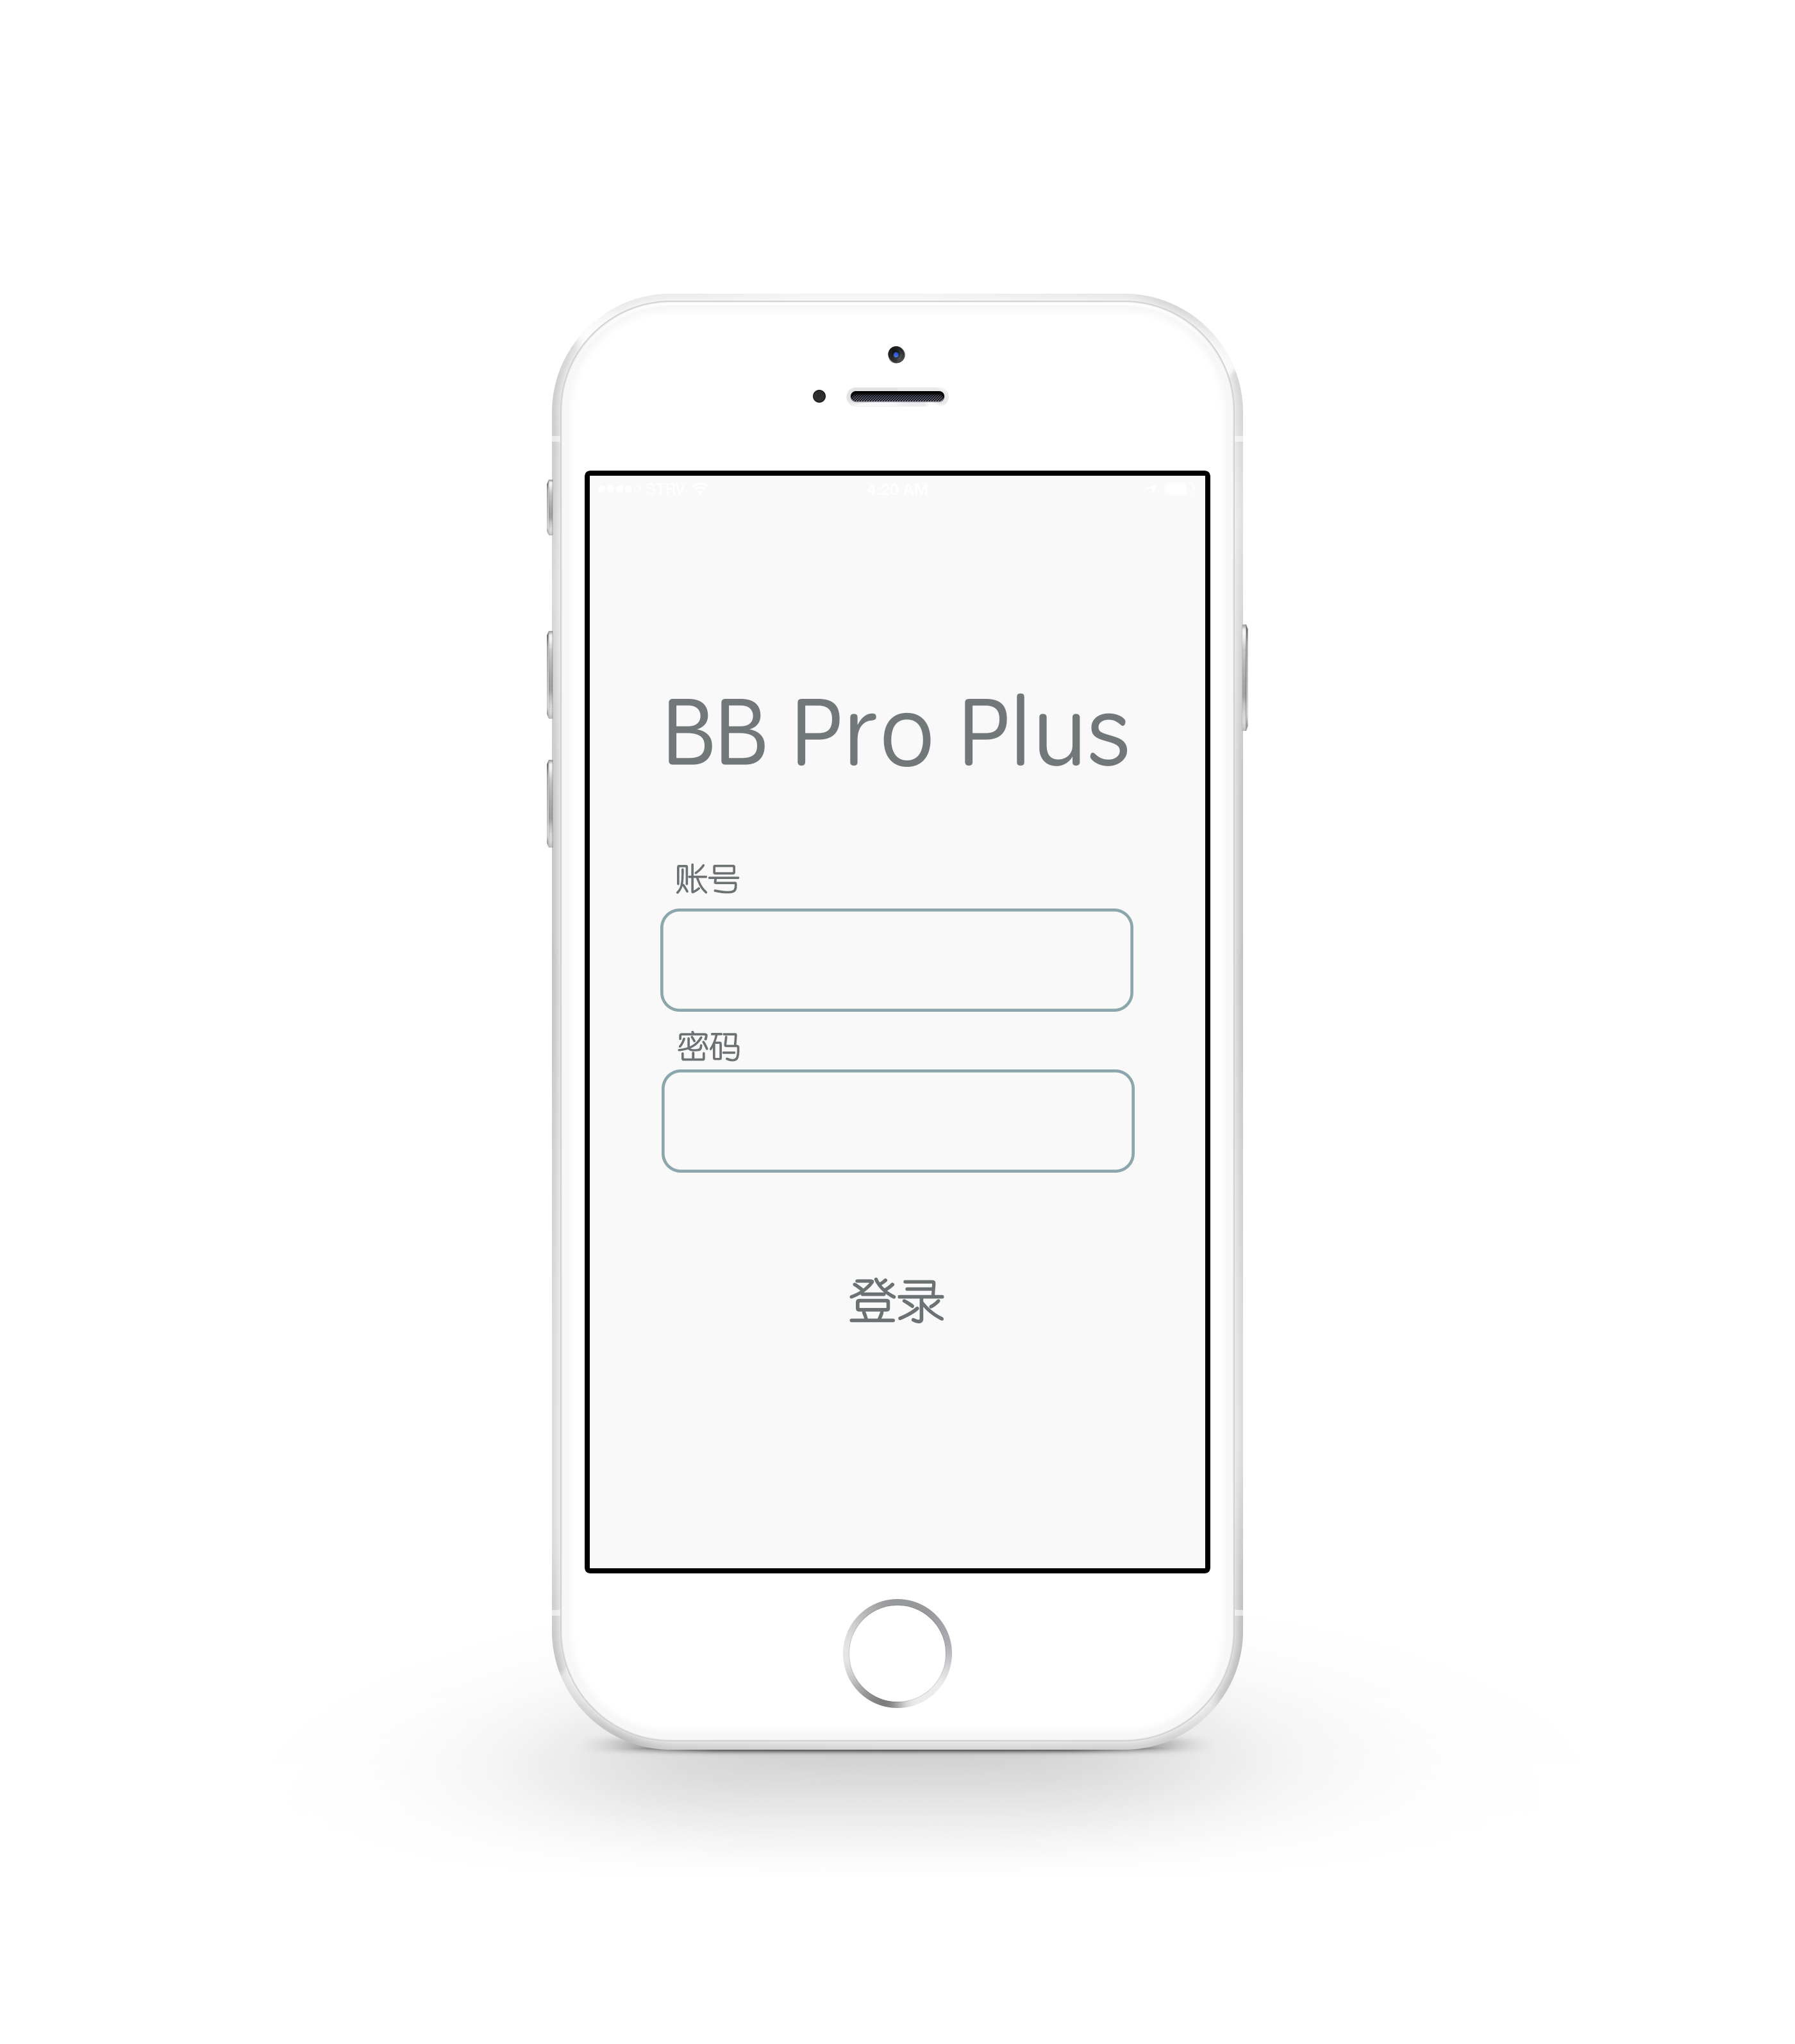
\includegraphics[width=11cm]{login}
\caption{登陆界面}
\end{figure}
\section{菜单界面}
\begin{figure}[H]
\centering
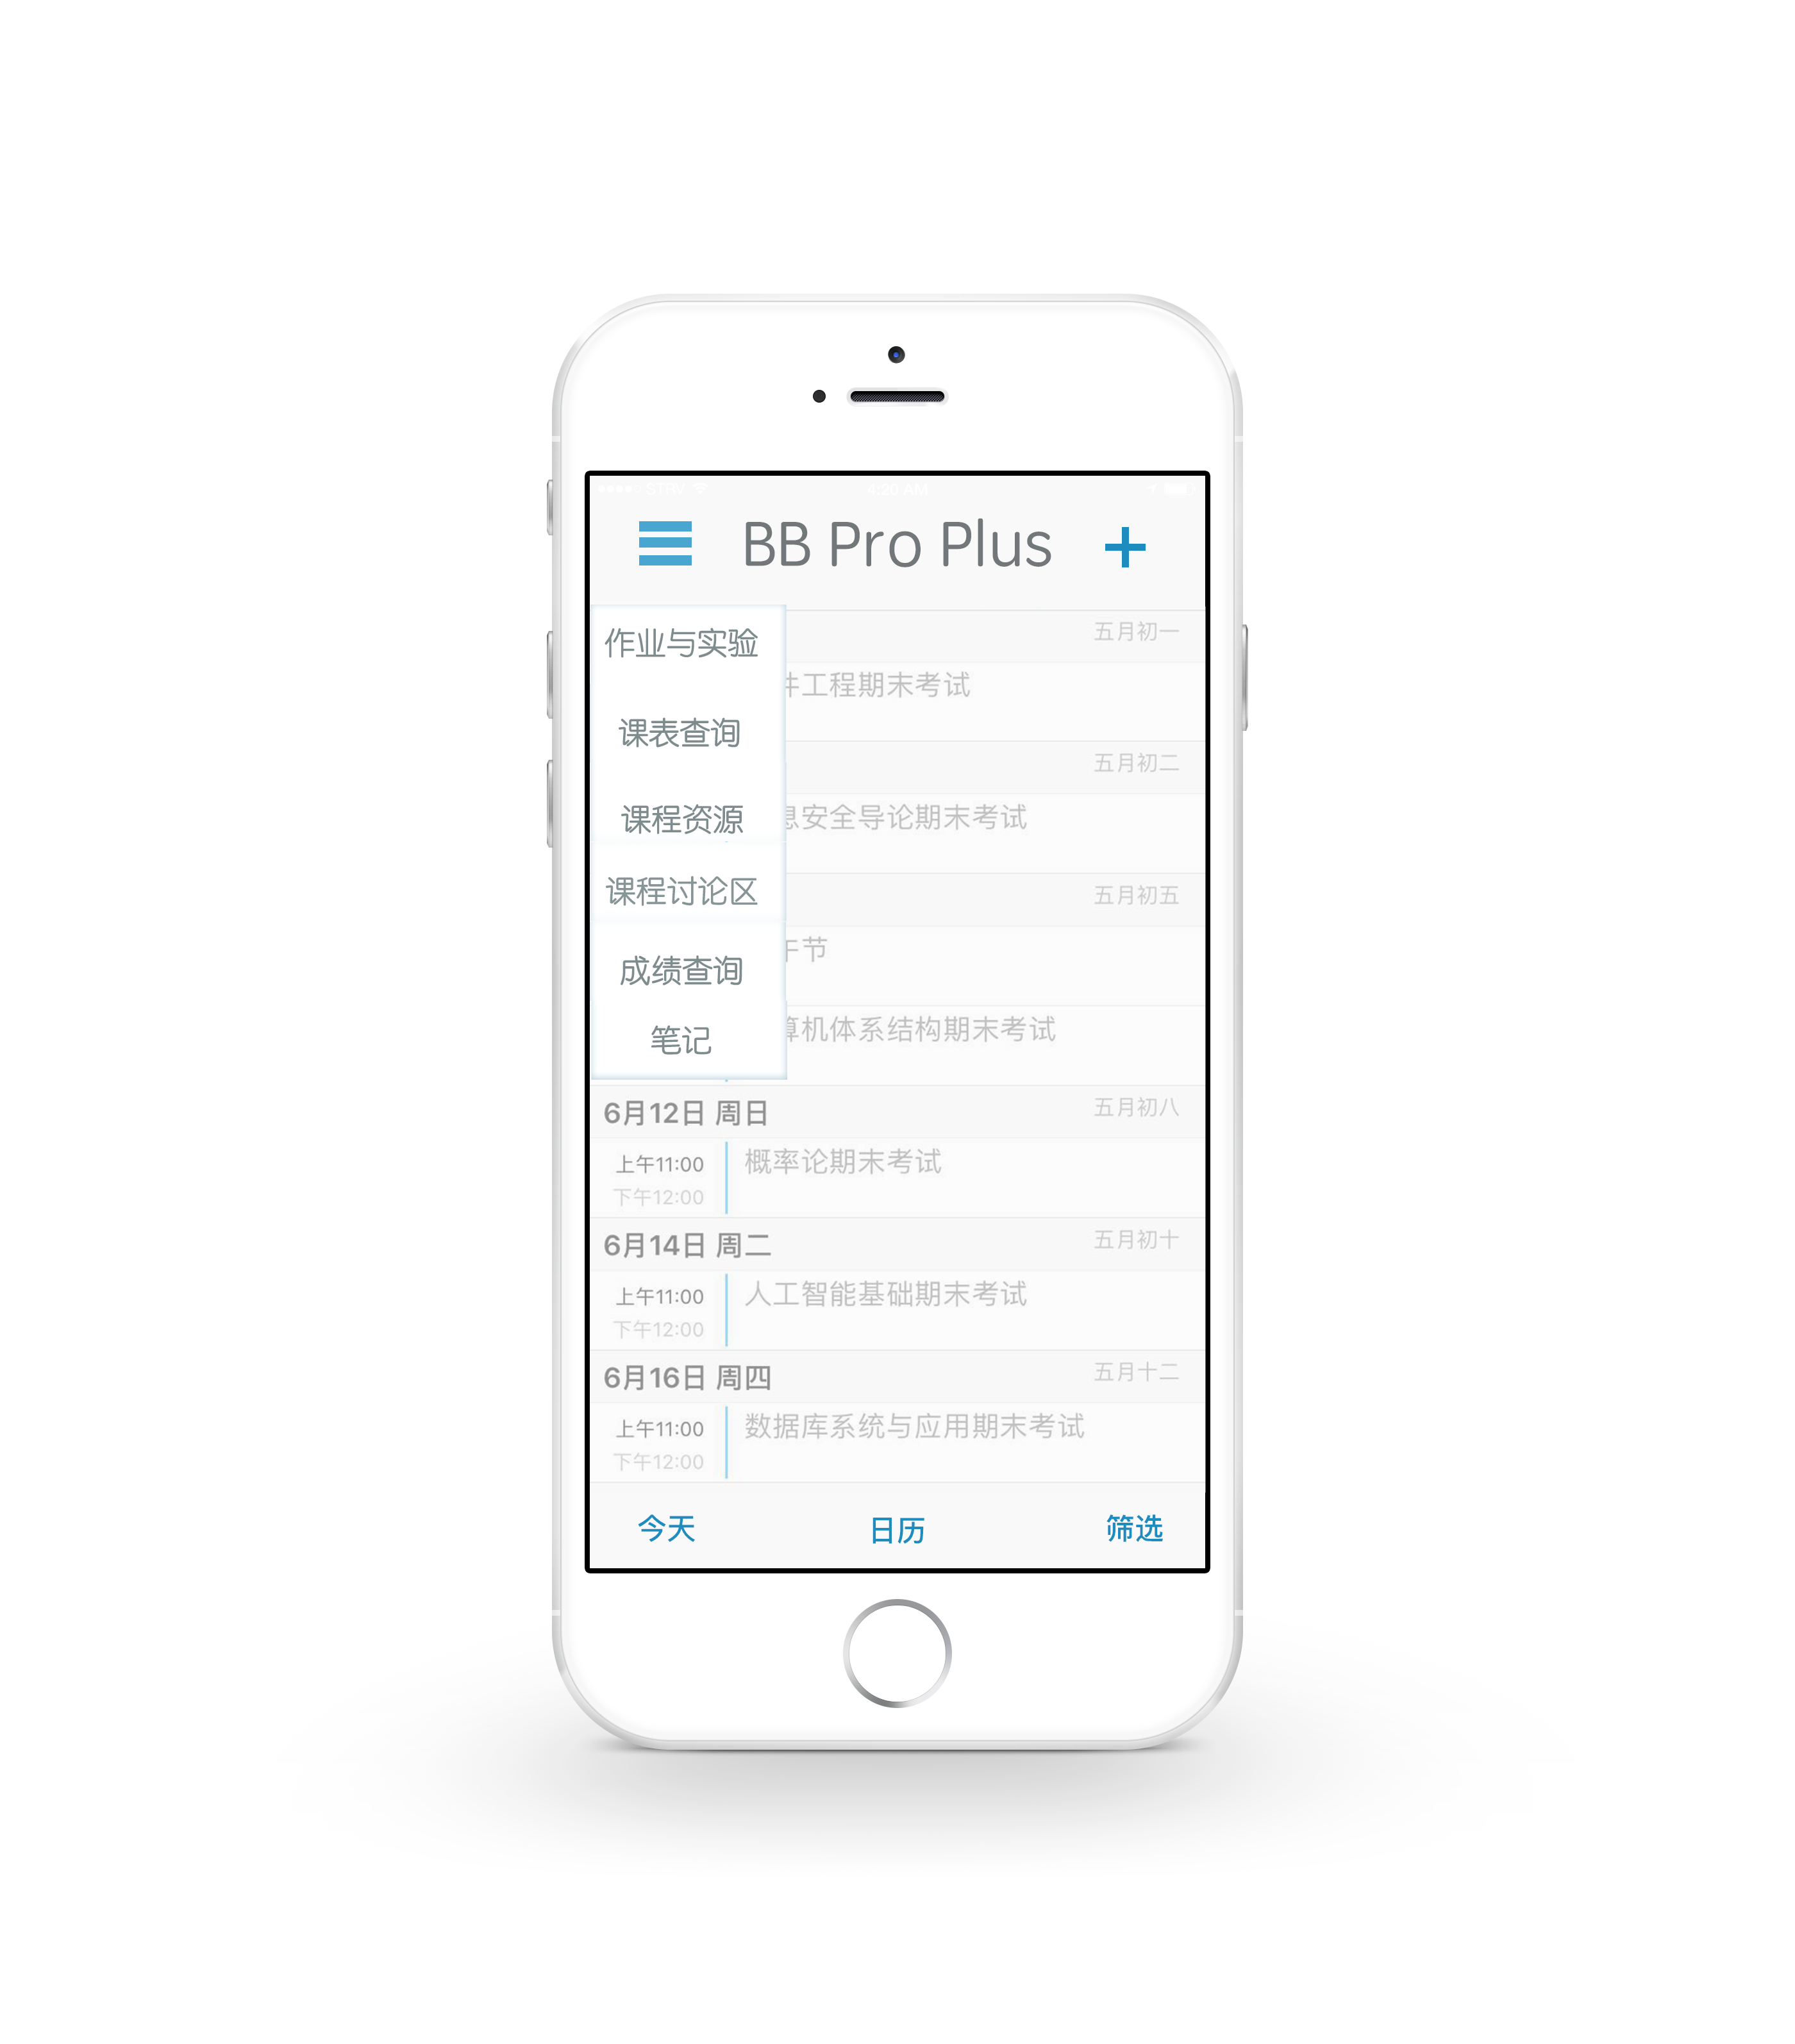
\includegraphics[width=11cm]{menu}
\caption{菜单界面}
\end{figure}
\section{作业实验界面}
\begin{figure}[H]
\centering
\subfigure[作业实验详情]{
\begin{minipage}{8cm}
\centering
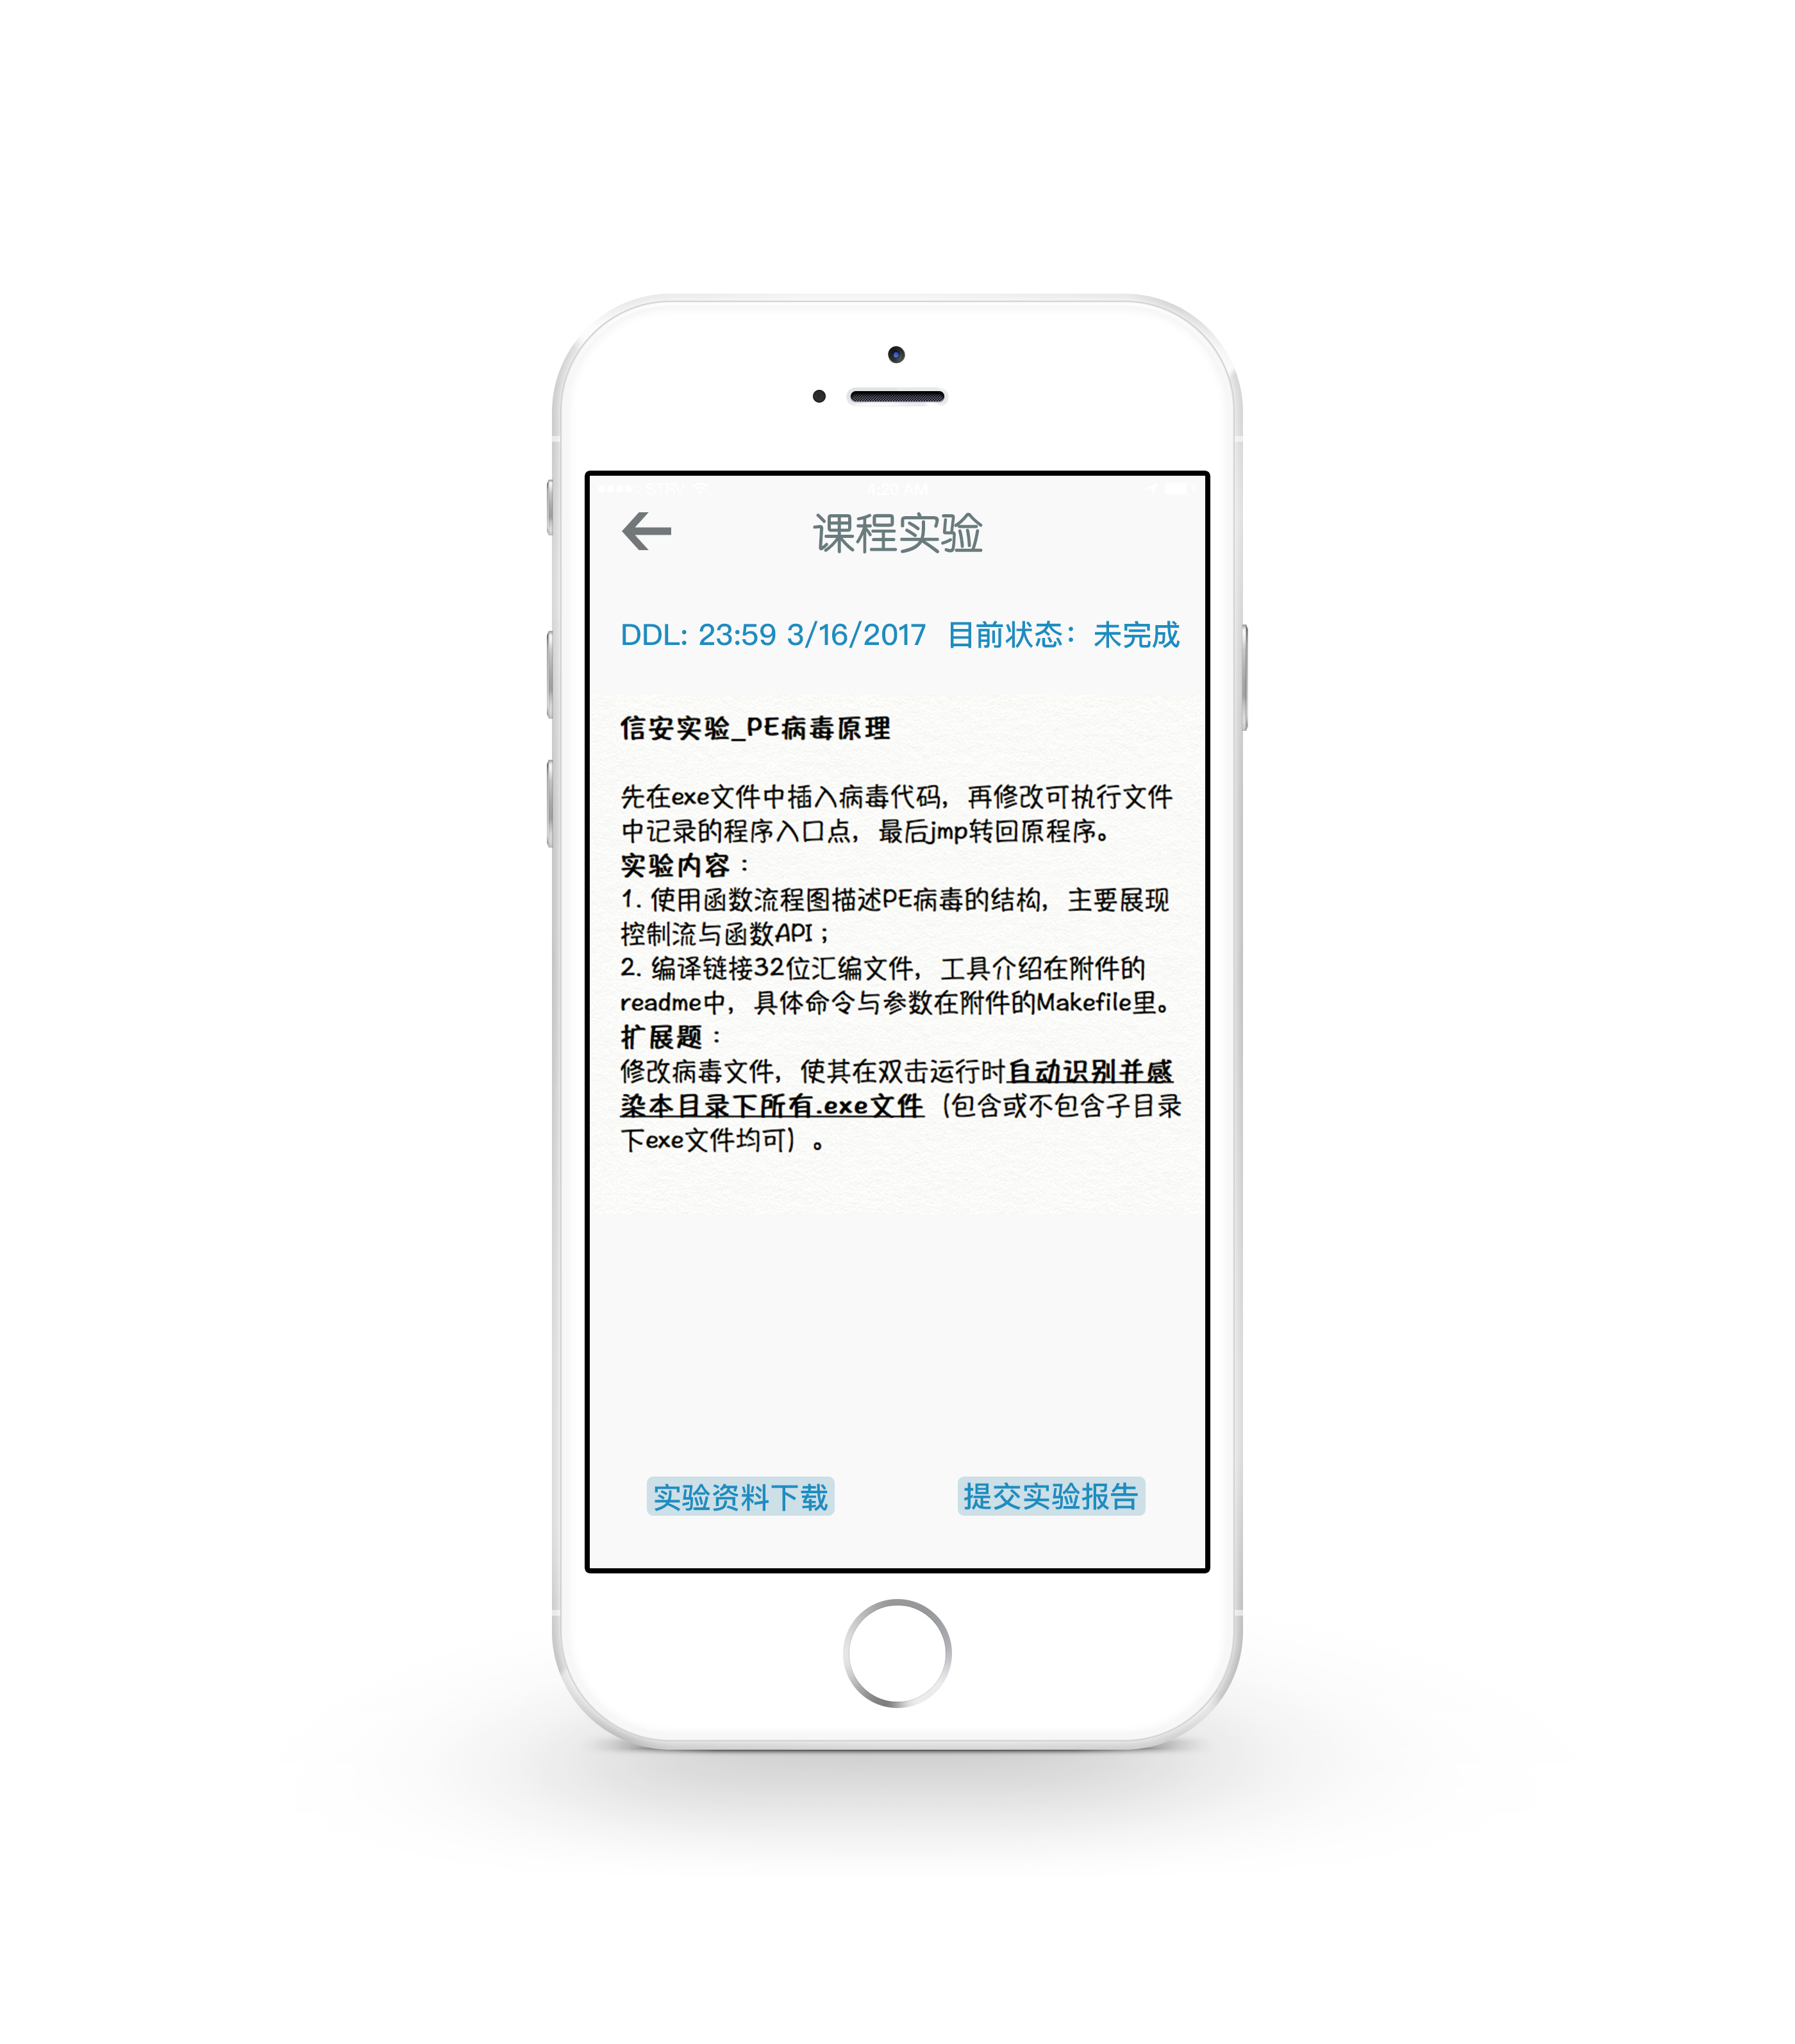
\includegraphics[width=8cm]{experiment_detail}
\end{minipage}
}
\subfigure[作业实验列表]{
\begin{minipage}{8cm}
\centering
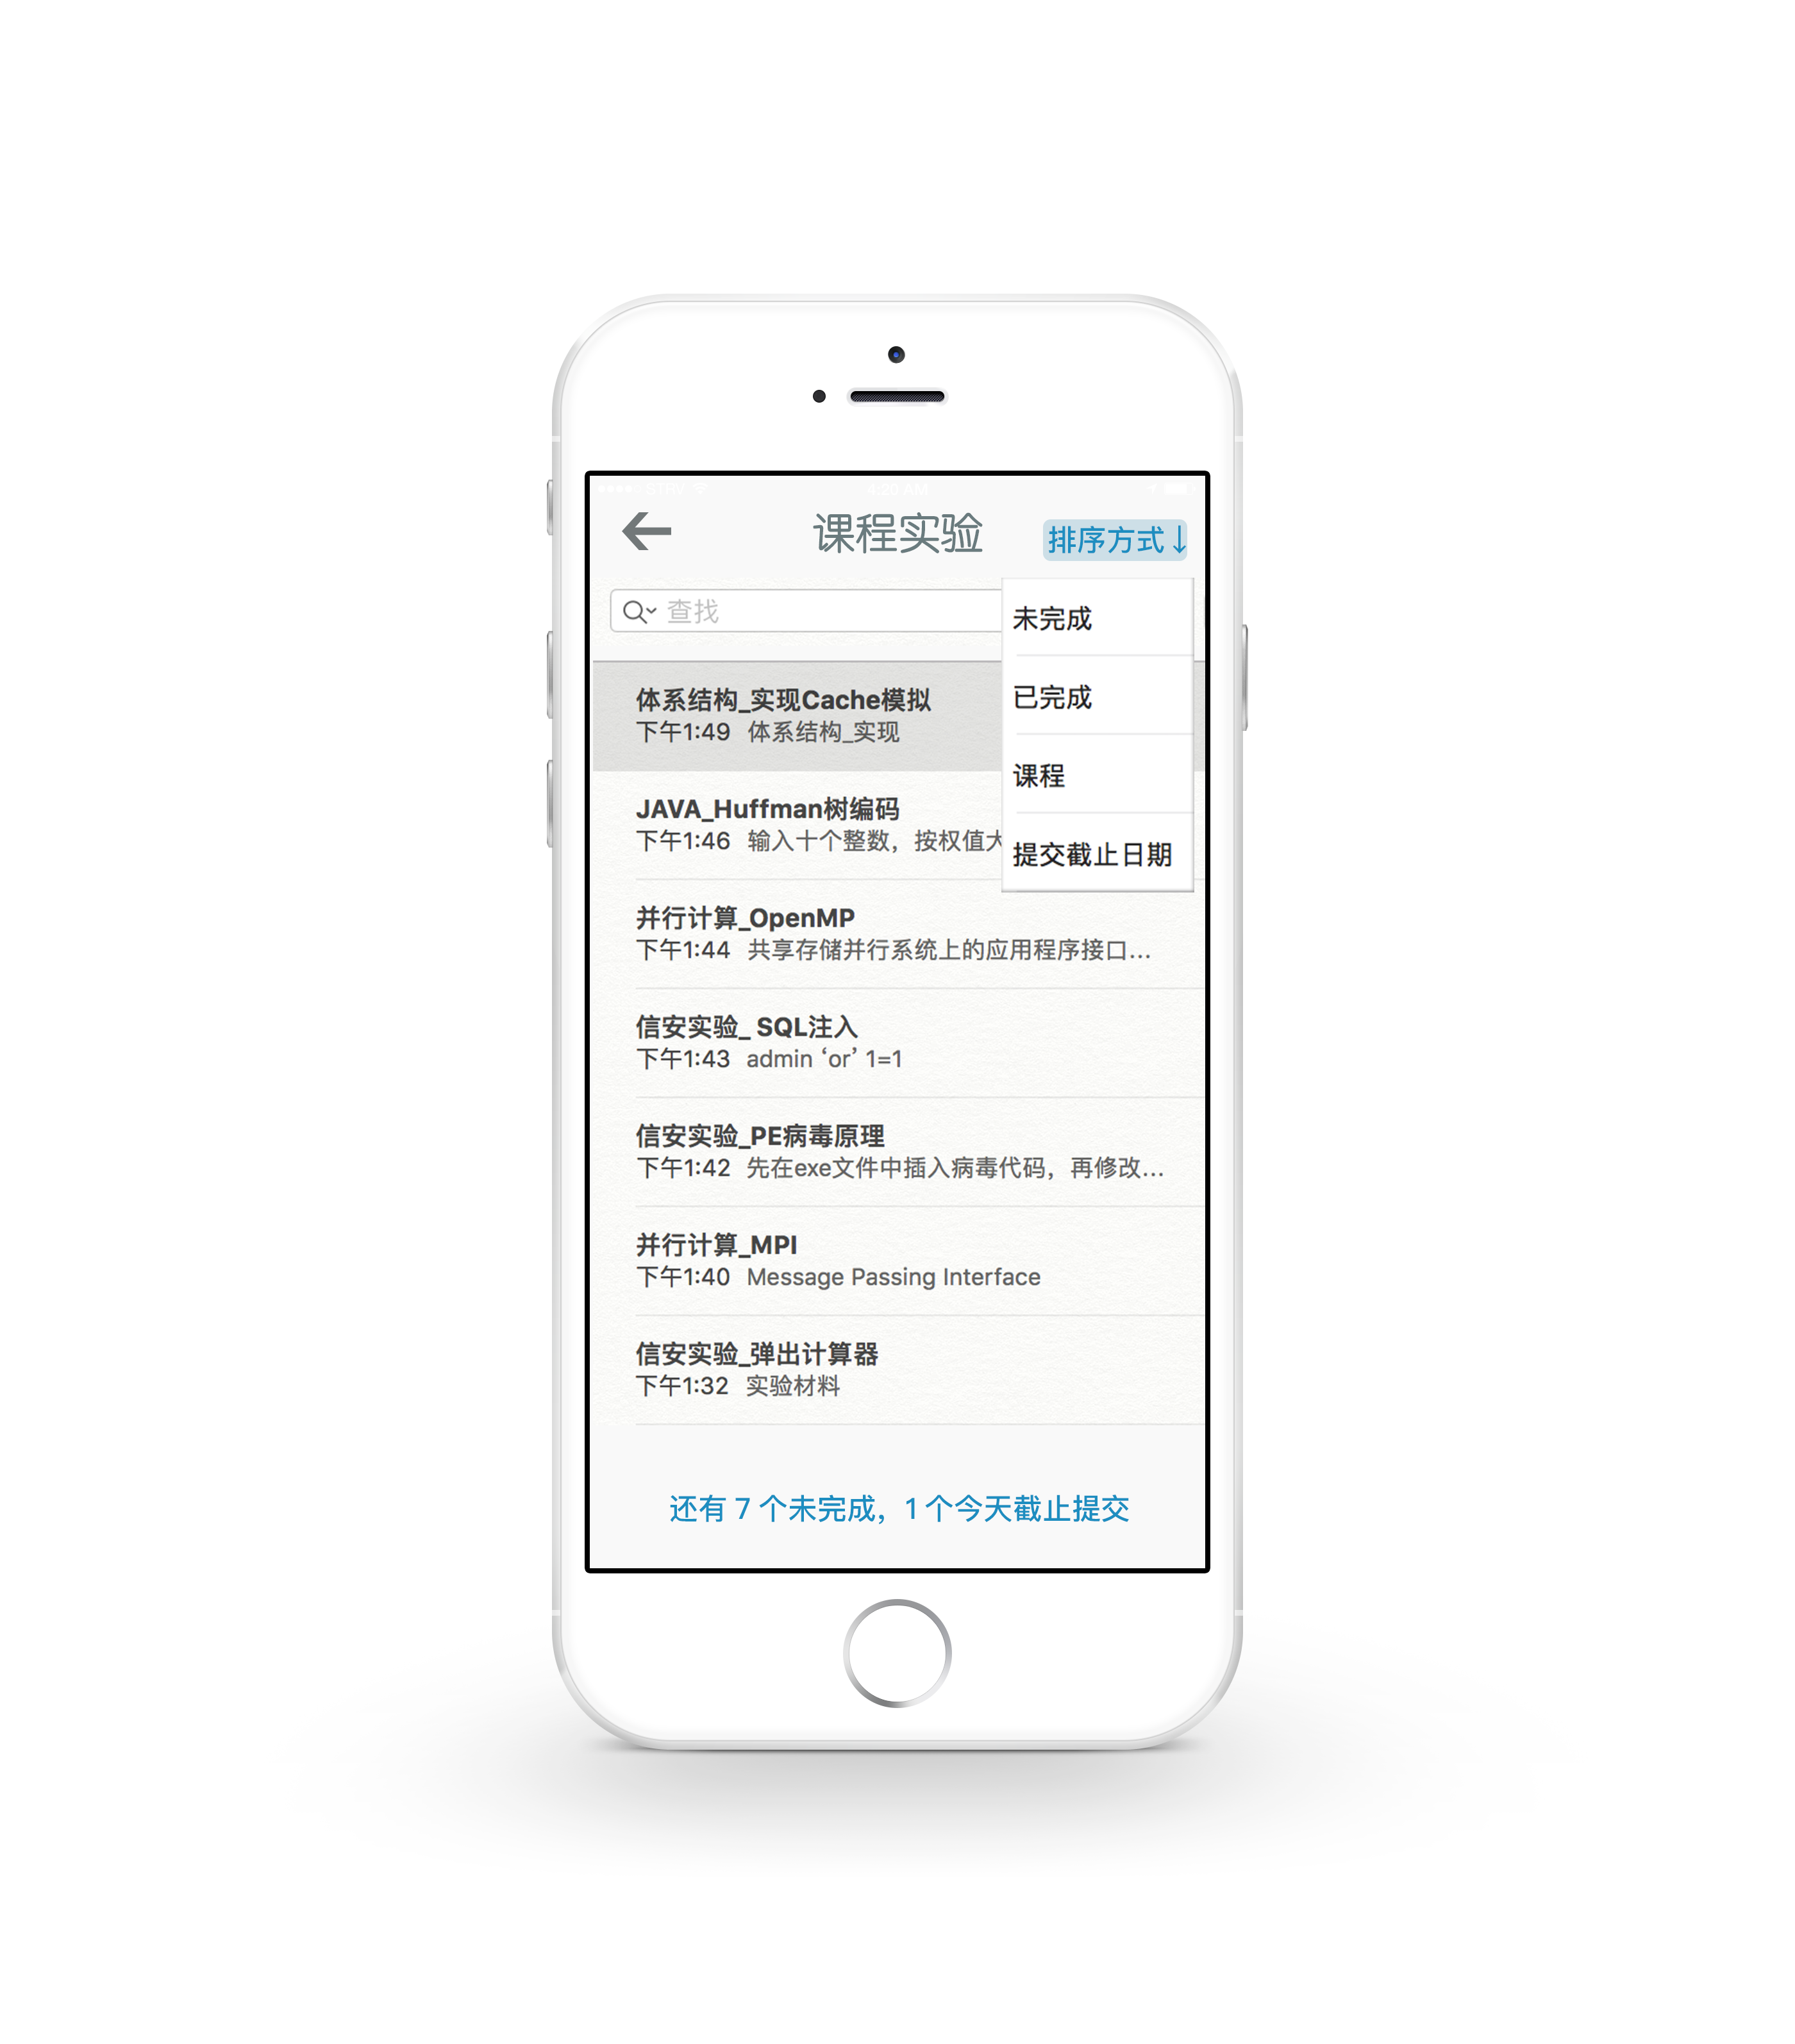
\includegraphics[width=8cm]{experiment_list}
\end{minipage}
}
\caption{作业实验界面}
\end{figure}
\section{日程管理界面}
\begin{figure}[H]
\centering
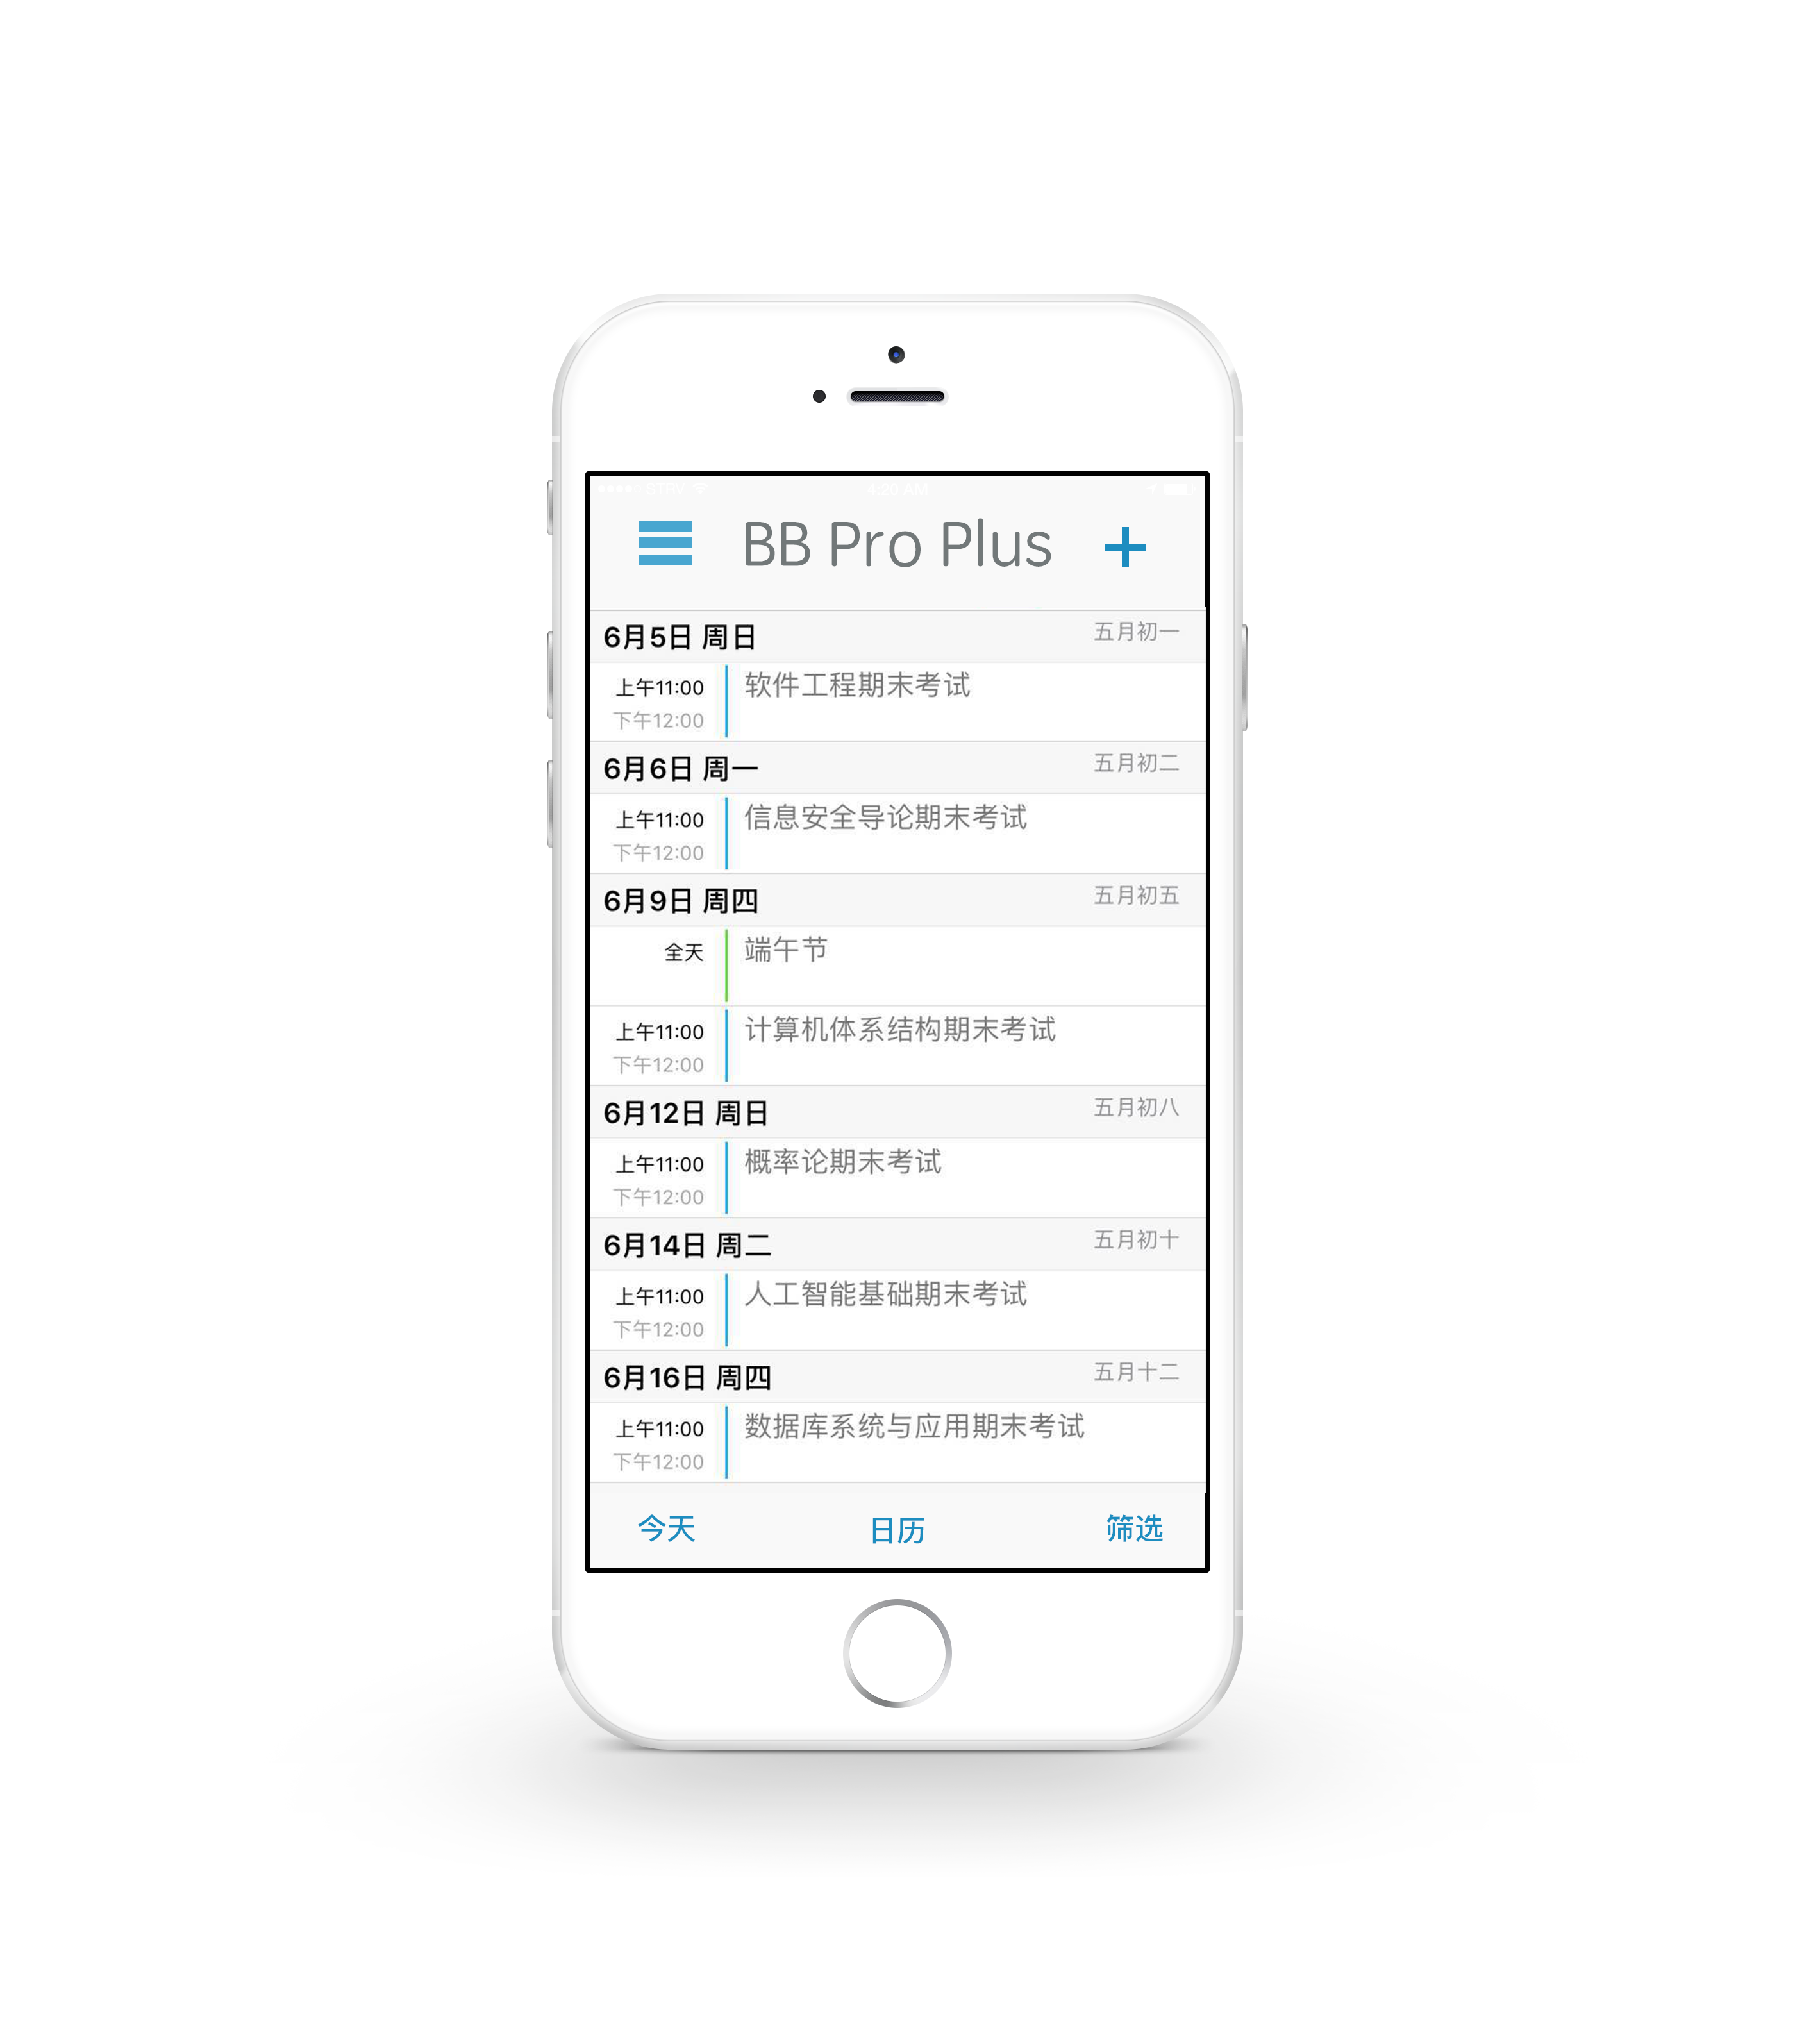
\includegraphics[width=11cm]{ddl}
\caption{日程管理界面}
\end{figure}
\section{讨论区界面}
\begin{figure}[H]
\centering
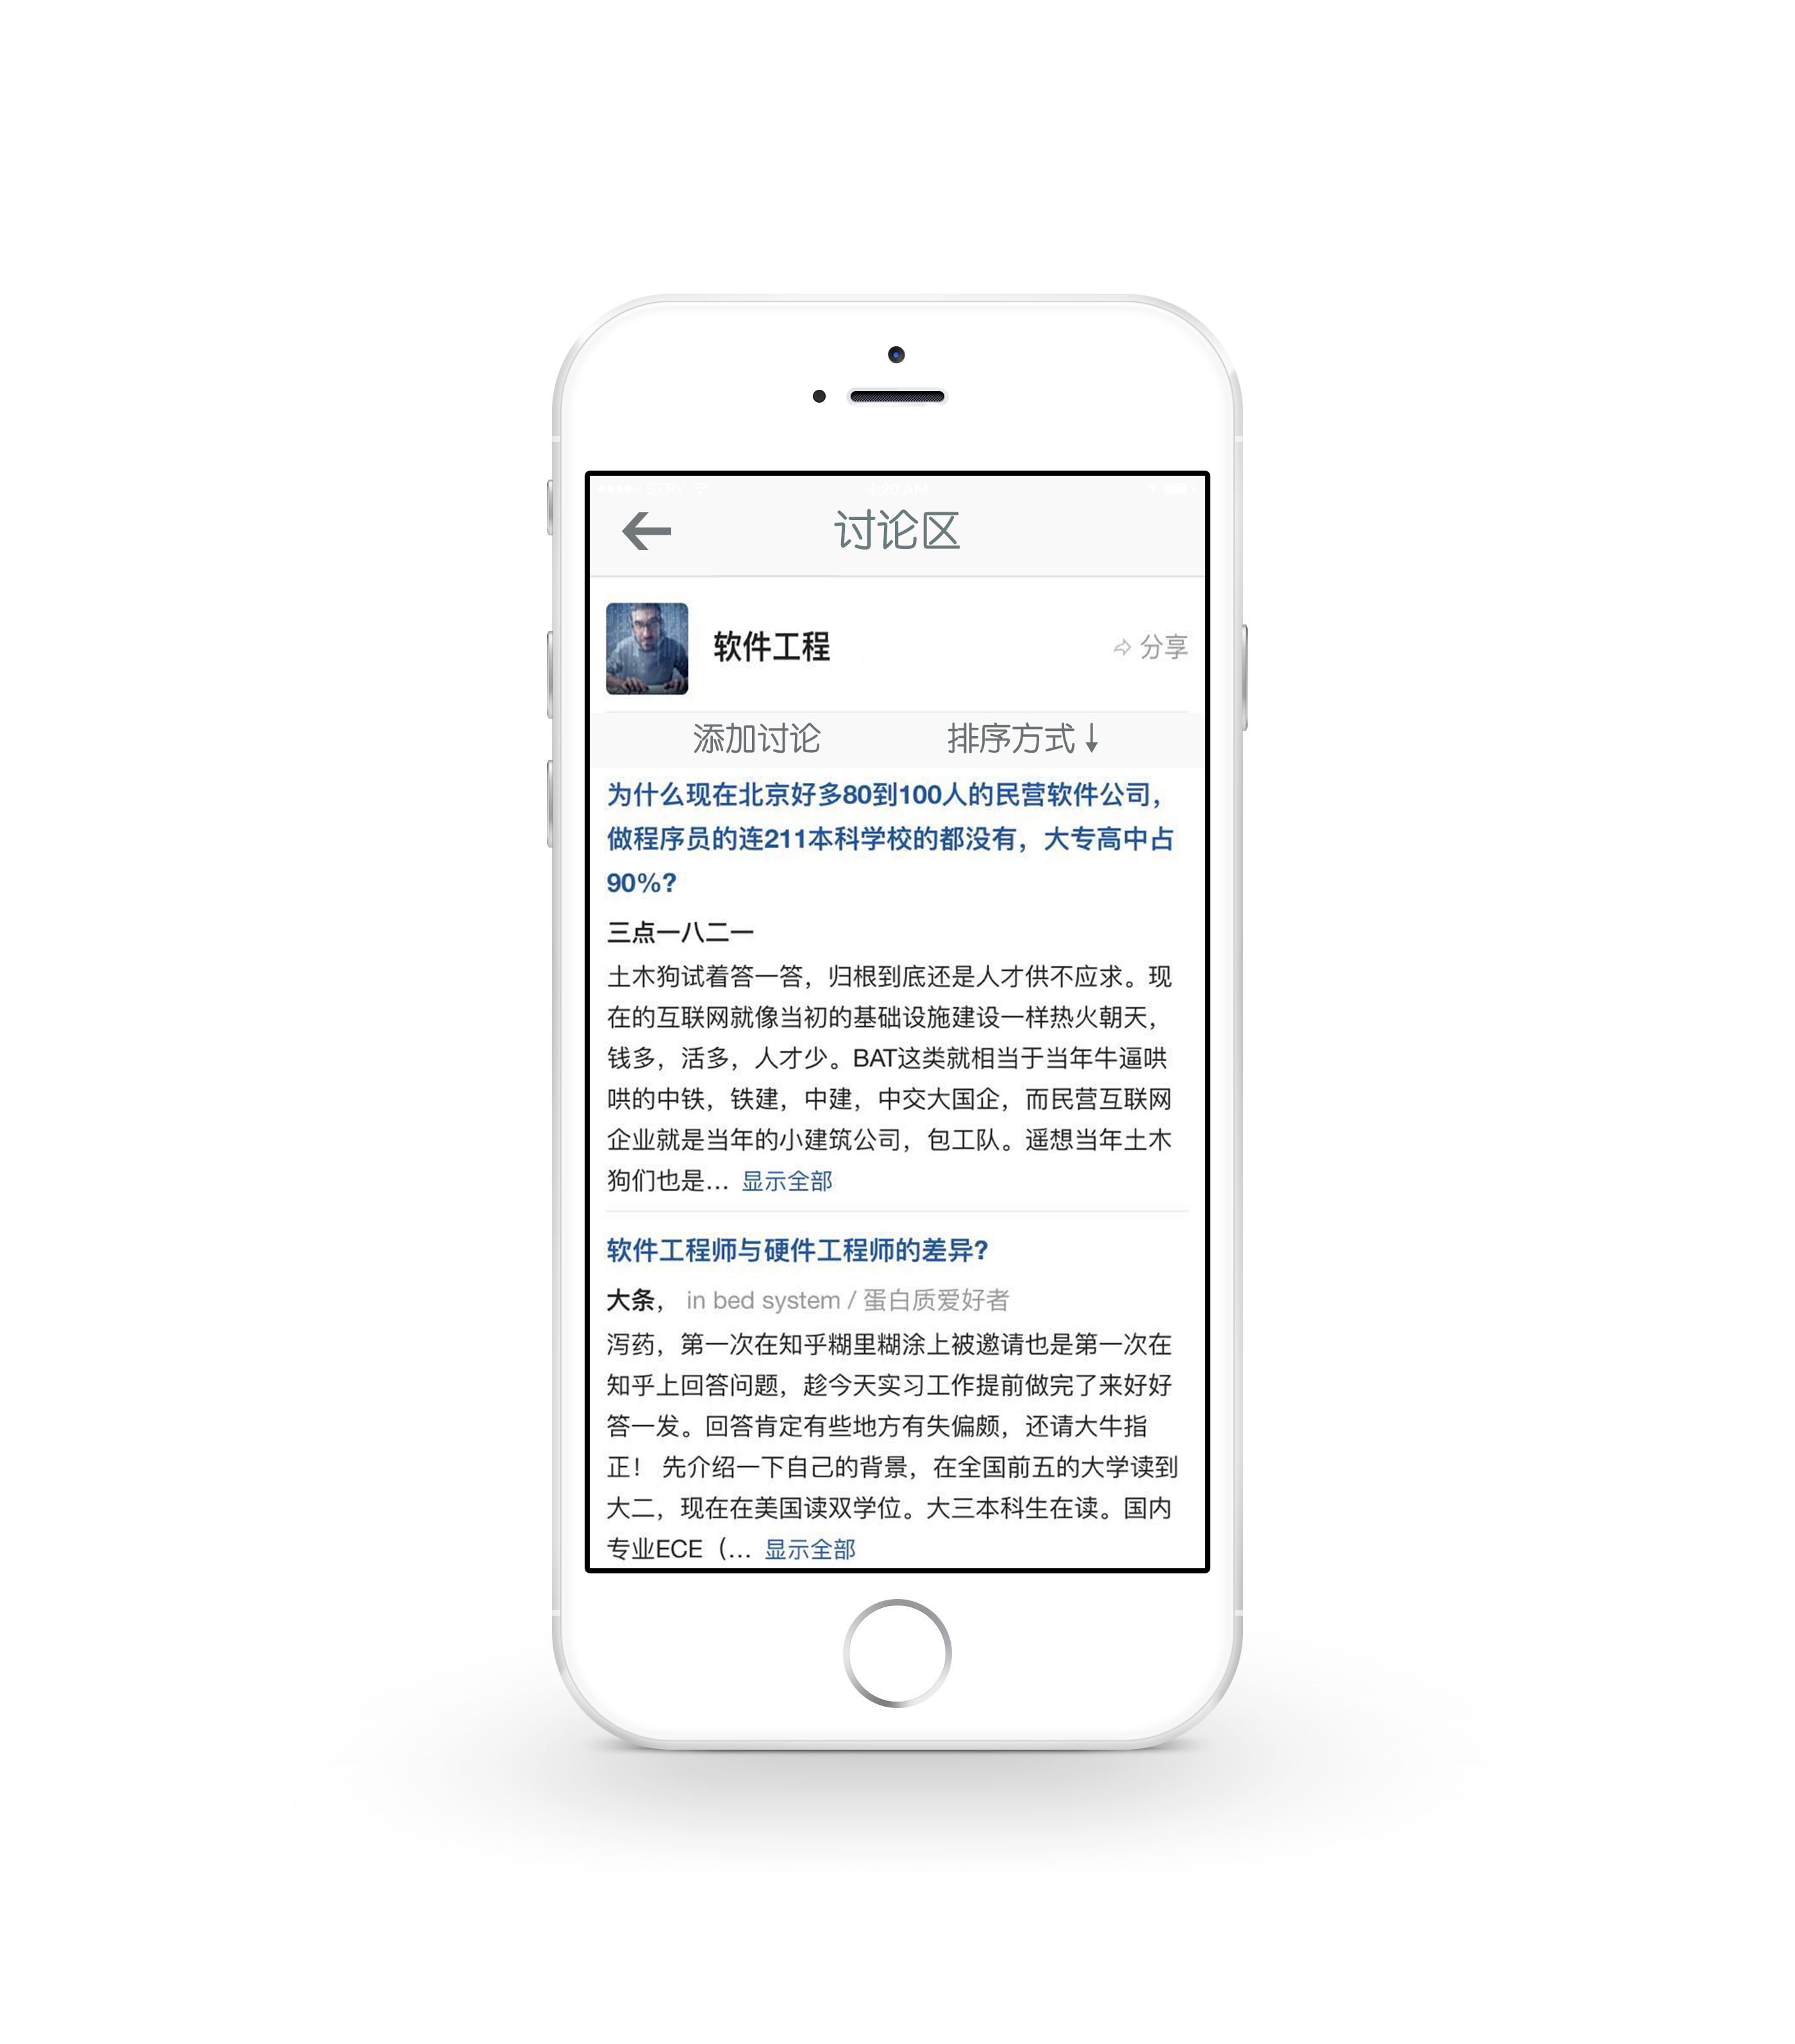
\includegraphics[width=11cm]{Discussion}
\caption{讨论区界面}
\end{figure}
\section{笔记界面}
\begin{figure}[H]
\centering
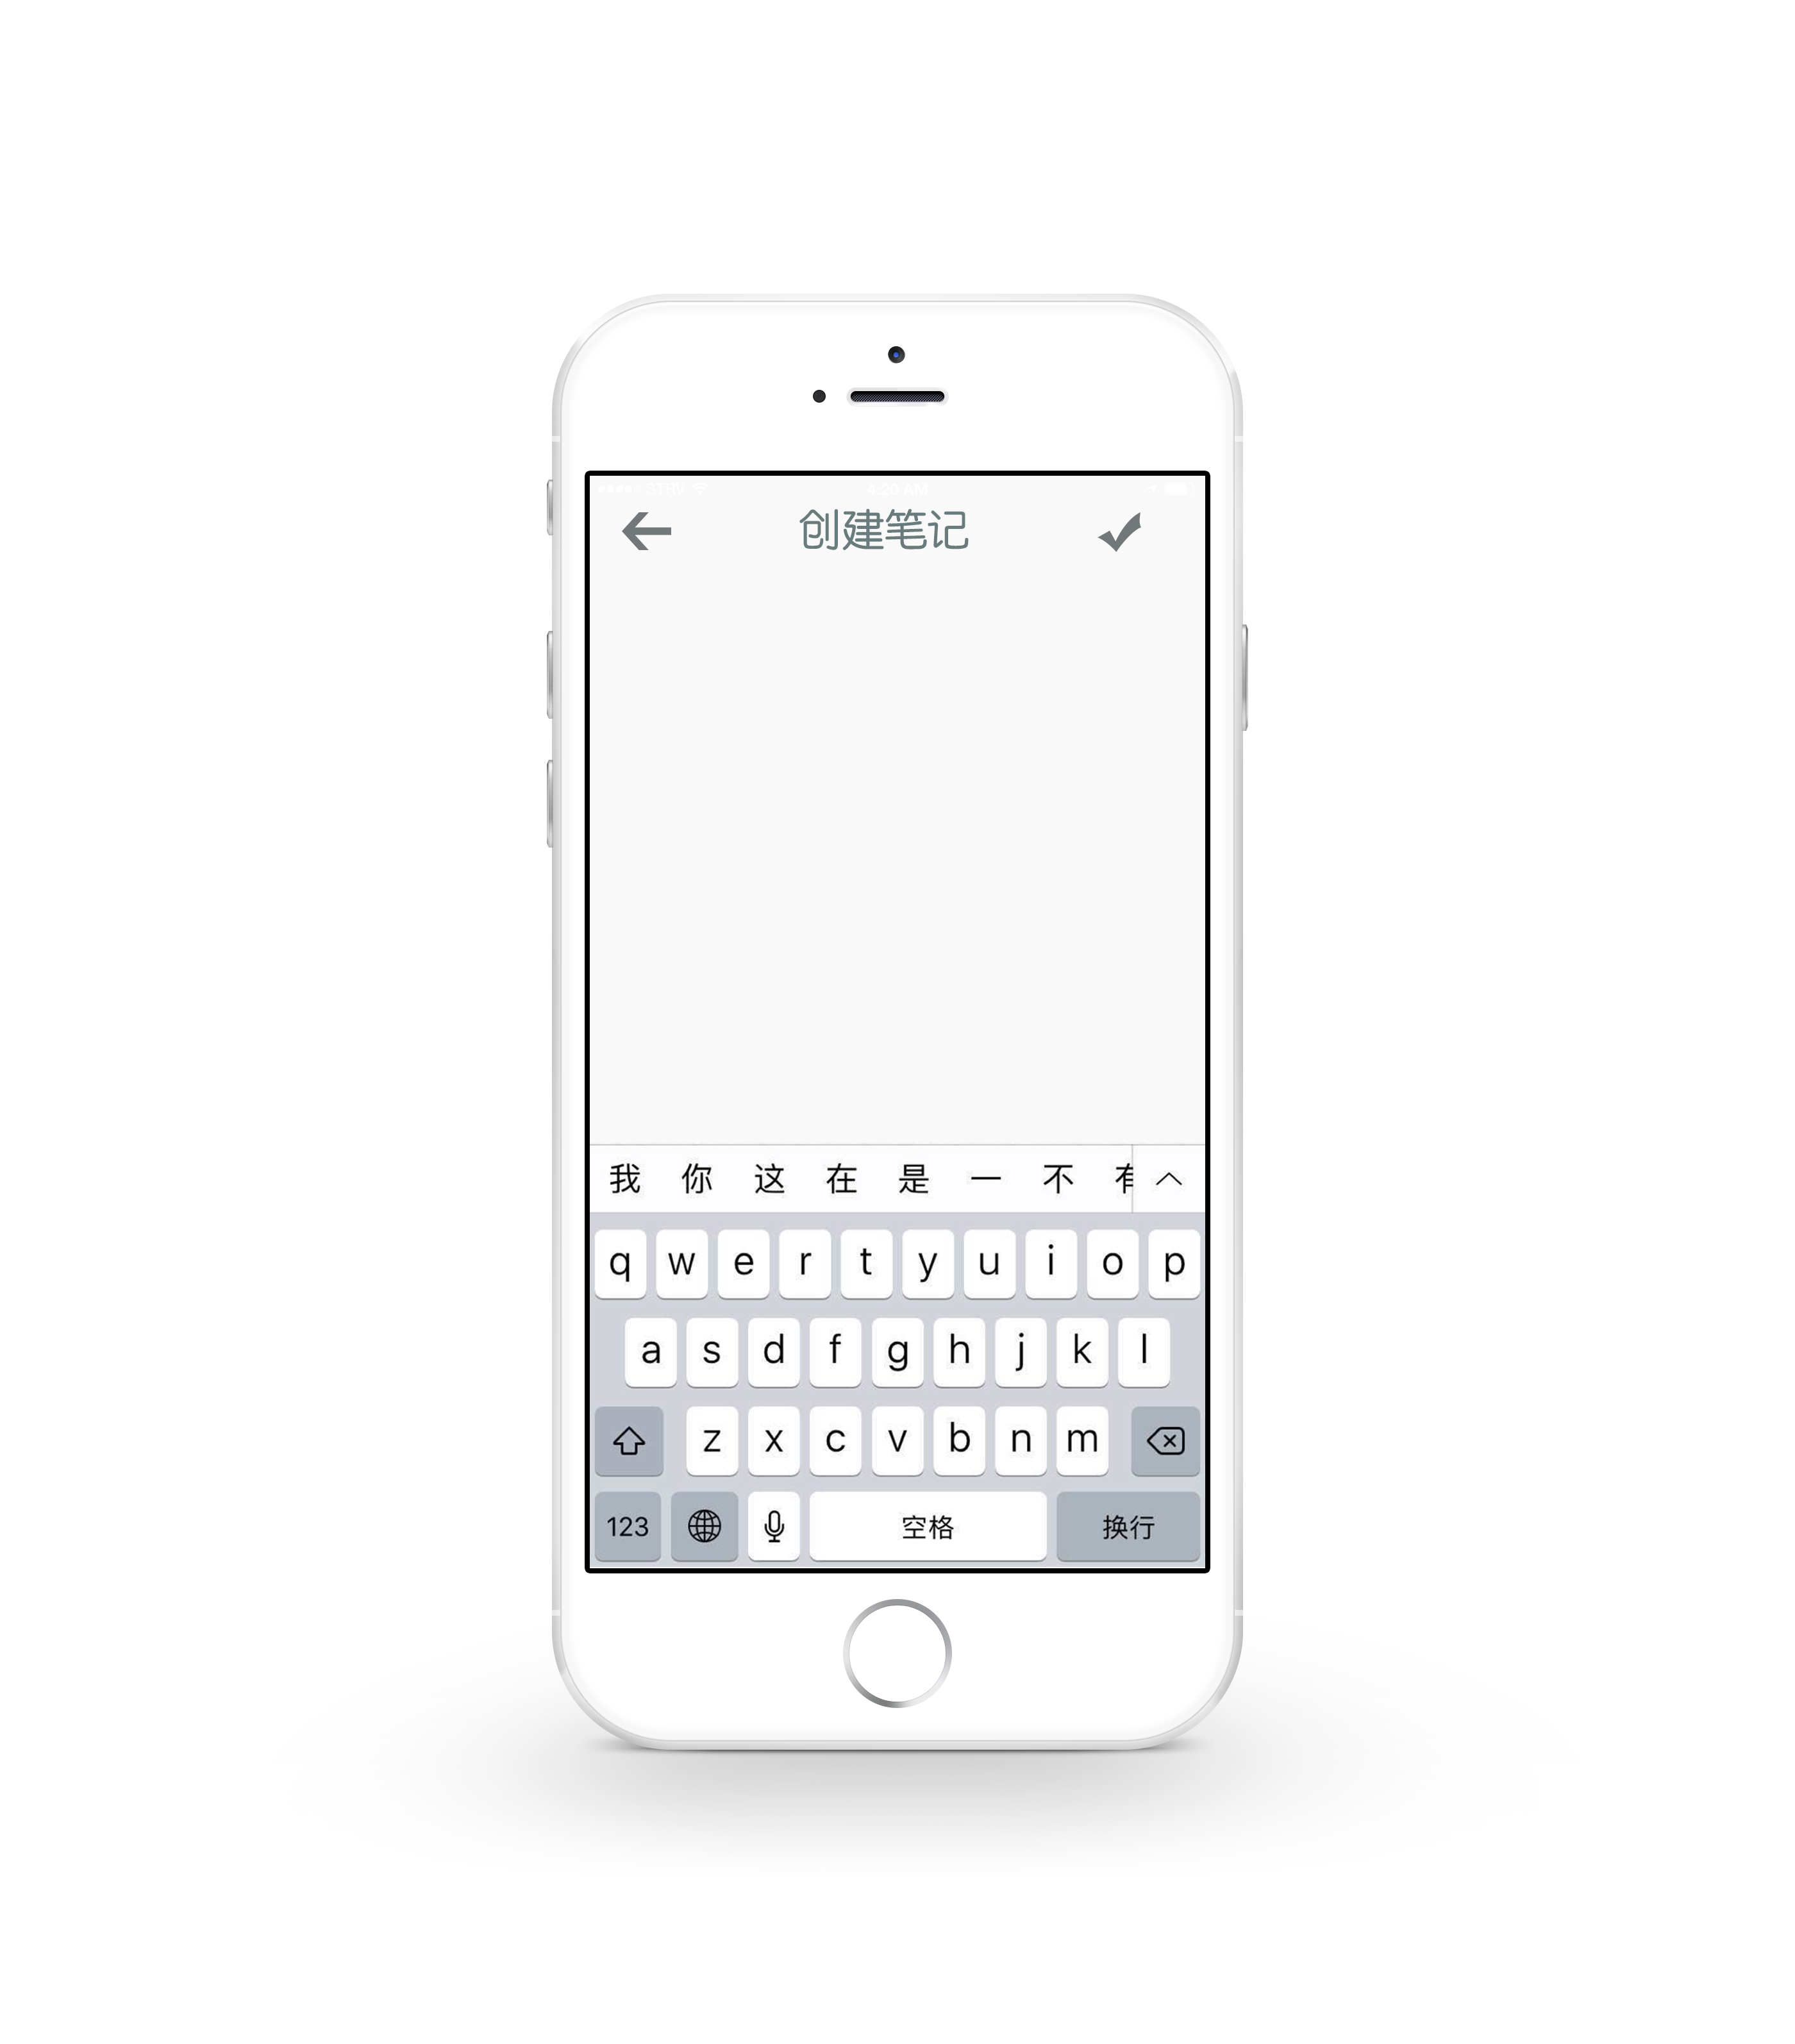
\includegraphics[width=11cm]{CreateNote}
\caption{笔记界面}
\end{figure}

\chapter{出错处理设计}
\section{数据库出错处理}
多重备份时,应采取何种策略,先利用哪一份备份;系统是否暂停服务等。

\section{某模块失效处理}
是否整个系统暂停服务,还是维持最小服务状态、如何尽快恢复服务还是删库跑路等。
\chapter{安全保密设计}
使用RBAC模型,不同的用户拥有不同的访问数据库权限。

不同类型的数据采用不同的传输方式,作业等数据不采用加密传输。

对于成绩信息,采用RSA加密传输,使用512位的密钥。


\chapter{维护设计}

定时备份。
\begin{itemize}
\item 日志备份1小时一次

\item 增量备份一天一次

\item 完全备份一星期一次
\end{itemize}

监视系统运行状态,出现异常时立即通知管理员。

定期如一学期一次清理已经过期的文件等,清理磁盘空间。


\chapter{图片}
本章展示图片相关用法。

\section{示例}
\begin{figure}[ht]
\centering

\includegraphics[width=10cm]{ustc_logo_fig}
\caption{测试图片} \label{fig:figure1}
\end{figure}

\section{带图注的图}
\begin{figure}[ht]
\centering

\includegraphics[width=10cm]{ustc_logo_fig}
\caption{带图注的图片}\label{fig:noted-figure}
\note{the solid lines represent the time histogram of the spontaneous activities of an old monkey cell(gray) and a young monkey cell (black). The bin-width is 1}
\end{figure}

\chapter{表格}

\section{A Simple Table}
\begin{table}[htbp]
\centering
\caption{这里是表的标题} \label{tab:simpletable}
\begin{tabular}{|c|c|}
    \hline
    a & b \\
    \hline
    c & d \\
    \hline
\end{tabular}
\note{这里是表的注释}
\end{table}

\section{长表格}
\begin{longtable}{ccc}
% 首页表头
\caption[长表格演示]{长表格演示} \label{tab:longtable} \\
\toprule[1.5pt]
名称  & 说明 & 备注\\
\midrule[1pt]
\endfirsthead
% 续页表头
\caption[]{长表格演示(续)} \\
\toprule[1.5pt]
名称  & 说明 & 备注 \\
\midrule[1pt]
\endhead
% 首页表尾
\hline
\multicolumn{3}{r}{\small 续下页}
\endfoot
% 续页表尾
\bottomrule[1.5pt]
\endlastfoot

AAAAAAAAAAAA   &   BBBBBBBBBBB   &   CCCCCCCCCCCCCC   \\
AAAAAAAAAAAA   &   BBBBBBBBBBB   &   CCCCCCCCCCCCCC   \\
AAAAAAAAAAAA   &   BBBBBBBBBBB   &   CCCCCCCCCCCCCC   \\
AAAAAAAAAAAA   &   BBBBBBBBBBB   &   CCCCCCCCCCCCCC   \\
AAAAAAAAAAAA   &   BBBBBBBBBBB   &   CCCCCCCCCCCCCC   \\
AAAAAAAAAAAA   &   BBBBBBBBBBB   &   CCCCCCCCCCCCCC   \\
AAAAAAAAAAAA   &   BBBBBBBBBBB   &   CCCCCCCCCCCCCC   \\
AAAAAAAAAAAA   &   BBBBBBBBBBB   &   CCCCCCCCCCCCCC   \\
AAAAAAAAAAAA   &   BBBBBBBBBBB   &   CCCCCCCCCCCCCC   \\
AAAAAAAAAAAA   &   BBBBBBBBBBB   &   CCCCCCCCCCCCCC   \\
AAAAAAAAAAAA   &   BBBBBBBBBBB   &   CCCCCCCCCCCCCC   \\
AAAAAAAAAAAA   &   BBBBBBBBBBB   &   CCCCCCCCCCCCCC   \\
AAAAAAAAAAAA   &   BBBBBBBBBBB   &   CCCCCCCCCCCCCC   \\
AAAAAAAAAAAA   &   BBBBBBBBBBB   &   CCCCCCCCCCCCCC   \\
AAAAAAAAAAAA   &   BBBBBBBBBBB   &   CCCCCCCCCCCCCC   \\
AAAAAAAAAAAA   &   BBBBBBBBBBB   &   CCCCCCCCCCCCCC   \\
AAAAAAAAAAAA   &   BBBBBBBBBBB   &   CCCCCCCCCCCCCC   \\
AAAAAAAAAAAA   &   BBBBBBBBBBB   &   CCCCCCCCCCCCCC   \\
AAAAAAAAAAAA   &   BBBBBBBBBBB   &   CCCCCCCCCCCCCC   \\
AAAAAAAAAAAA   &   BBBBBBBBBBB   &   CCCCCCCCCCCCCC   \\
AAAAAAAAAAAA   &   BBBBBBBBBBB   &   CCCCCCCCCCCCCC   \\
AAAAAAAAAAAA   &   BBBBBBBBBBB   &   CCCCCCCCCCCCCC   \\
AAAAAAAAAAAA   &   BBBBBBBBBBB   &   CCCCCCCCCCCCCC   \\
AAAAAAAAAAAA   &   BBBBBBBBBBB   &   CCCCCCCCCCCCCC   \\
AAAAAAAAAAAA   &   BBBBBBBBBBB   &   CCCCCCCCCCCCCC   \\
AAAAAAAAAAAA   &   BBBBBBBBBBB   &   CCCCCCCCCCCCCC   \\
AAAAAAAAAAAA   &   BBBBBBBBBBB   &   CCCCCCCCCCCCCC   \\
AAAAAAAAAAAA   &   BBBBBBBBBBB   &   CCCCCCCCCCCCCC   \\
AAAAAAAAAAAA   &   BBBBBBBBBBB   &   CCCCCCCCCCCCCC   \\
AAAAAAAAAAAA   &   BBBBBBBBBBB   &   CCCCCCCCCCCCCC   \\
AAAAAAAAAAAA   &   BBBBBBBBBBB   &   CCCCCCCCCCCCCC   \\
AAAAAAAAAAAA   &   BBBBBBBBBBB   &   CCCCCCCCCCCCCC   \\
AAAAAAAAAAAA   &   BBBBBBBBBBB   &   CCCCCCCCCCCCCC   \\
AAAAAAAAAAAA   &   BBBBBBBBBBB   &   CCCCCCCCCCCCCC   \\
AAAAAAAAAAAA   &   BBBBBBBBBBB   &   CCCCCCCCCCCCCC   \\
AAAAAAAAAAAA   &   BBBBBBBBBBB   &   CCCCCCCCCCCCCC   \\
\end{longtable}

\chapter{算法环境}
模板中使用 \texttt{algorithm2e} 宏包实现算法环境。关于该宏包的具体用法,
请阅读宏包的官方文档。

\begin{algorithm}[htbp]
\SetAlgoLined
\KwData{this text}
\KwResult{how to write algorithm with \LaTeX2e }

initialization\;
\While{not at end of this document}{
    read current\;
    \eIf{understand}{
        go to next section\;
        current section becomes this one\;
    }{
        go back to the beginning of current section\;
    }
}
\caption{算法示例1}
\label{algo:algorithm1}
\end{algorithm}

\IncMargin{1em}
\begin{algorithm}
\SetKwData{Left}{left}\SetKwData{This}{this}\SetKwData{Up}{up}
\SetKwFunction{Union}{Union}\SetKwFunction{FindCompress}{FindCompress}
\SetKwInOut{Input}{input}\SetKwInOut{Output}{output}

\Input{A bitmap $Im$ of size $w\times l$}
\Output{A partition of the bitmap}
\BlankLine
\emph{special treatment of the first line}\;
\For{$i\leftarrow 2$ \KwTo $l$}{
    \emph{special treatment of the first element of line $i$}\;
    \For{$j\leftarrow 2$ \KwTo $w$}{\label{forins}
        \Left$\leftarrow$ \FindCompress{$Im[i,j-1]$}\;
        \Up$\leftarrow$ \FindCompress{$Im[i-1,]$}\;
        \This$\leftarrow$ \FindCompress{$Im[i,j]$}\;
        \If(\tcp*[h]{O(\Left,\This)==1}){\Left compatible with \This}{\label{lt}
            \lIf{\Left $<$ \This}{\Union{\Left,\This}}
            \lElse{\Union{\This,\Left}}
        }
        \If(\tcp*[f]{O(\Up,\This)==1}){\Up compatible with \This}{\label{ut}
        \lIf{\Up $<$ \This}{\Union{\Up,\This}}
        \tcp{\This is put under \Up to keep tree as flat as possible}\label{cmt}
        \lElse{\Union{\This,\Up}}\tcp*[h]{\This linked to \Up}\label{lelse}
        }
    }
    \lForEach{element $e$ of the line $i$}{\FindCompress{p}}
}
\caption{算法示例2}\label{algo_disjdecomp}
\label{alog:algorithm2}
\end{algorithm}\DecMargin{1em}

\chapter{代码环境}
模板中使用 \texttt{listings} 宏包实现代码环境。详细用法见宏包的官方说明文档。

以下是代码示例,可以在文中任意位置引用\autoref{first-code} 。
\begin{lstlisting}[language=C, caption=示例代码, label={code:first-code}]
#include <stdio.h>

int main( )
{
    printf("hello, world\n");
    return 0;
}
\end{lstlisting}

\chapter{引用文献标注}

\section{著者-出版年制标注法}

\noindent
\verb|\citestyle{ustcauthoryear}|
\citestyle{ustcauthoryear}

\noindent
\begin{tabular}{l@{\quad$\Rightarrow$\quad}l}
  \verb|\cite{knuth86a}| & \cite{knuth86a}\\
  \verb|\citet{knuth86a}| & \citet{knuth86a}\\
  \verb|\citet[chap.~2]{knuth86a}| & \citet[chap.~2]{knuth86a}\\[0.5ex]
  \verb|\citep{knuth86a}| & \citep{knuth86a}\\
  \verb|\citep[chap.~2]{knuth86a}| & \citep[chap.~2]{knuth86a}\\
  \verb|\citep[see][]{knuth86a}| & \citep[see][]{knuth86a}\\
  \verb|\citep[see][chap.~2]{knuth86a}| & \citep[see][chap.~2]{knuth86a}\\[0.5ex]
  \verb|\citet*{knuth86a}| & \citet*{knuth86a}\\
  \verb|\citep*{knuth86a}| & \citep*{knuth86a}\\
\end{tabular}

\noindent
\begin{tabular}{l@{\quad$\Rightarrow$\quad}l}
  \verb|\citet{knuth86a,tlc2}| & \citet{knuth86a,tlc2}\\
  \verb|\citep{knuth86a,tlc2}| & \citep{knuth86a,tlc2}\\
  \verb|\cite{knuth86a,knuth84}| & \cite{knuth86a,knuth84}\\
  \verb|\citet{knuth86a,knuth84}| & \citet{knuth86a,knuth84}\\
  \verb|\citep{knuth86a,knuth84}| & \citep{knuth86a,knuth84}\\
\end{tabular}

\section{顺序编码制标注法}

\noindent
\verb|\citestyle{ustcnumerical}|
\citestyle{ustcnumerical}

\noindent
\begin{tabular}{l@{\quad$\Rightarrow$\quad}l}
  \verb|\cite{knuth86a}| & \cite{knuth86a}\\
  \verb|\citet{knuth86a}| & \citet{knuth86a}\\
  \verb|\citet[chap.~2]{knuth86a}| & \citet[chap.~2]{knuth86a}\\[0.5ex]
  \verb|\citep{knuth86a}| & \citep{knuth86a}\\
  \verb|\citep[chap.~2]{knuth86a}| & \citep[chap.~2]{knuth86a}\\
  \verb|\citep[see][]{knuth86a}| & \citep[see][]{knuth86a}\\
  \verb|\citep[see][chap.~2]{knuth86a}| & \citep[see][chap.~2]{knuth86a}\\[0.5ex]
  \verb|\citet*{knuth86a}| & \citet*{knuth86a}\\
  \verb|\citep*{knuth86a}| & \citep*{knuth86a}\\
\end{tabular}

\noindent
\begin{tabular}{l@{\quad$\Rightarrow$\quad}l}
  \verb|\citet{knuth86a,tlc2}| & \citet{knuth86a,tlc2}\\
  \verb|\citep{knuth86a,tlc2}| & \citep{knuth86a,tlc2}\\
  \verb|\cite{knuth86a,knuth84}| & \cite{knuth86a,knuth84}\\
  \verb|\citet{knuth86a,knuth84}| & \citet{knuth86a,knuth84}\\
  \verb|\citep{knuth86a,knuth84}| & \citep{knuth86a,knuth84}\\
  \verb|\cite{knuth86a,knuth84,tlc2}| & \cite{knuth86a,knuth84,tlc2}\\
\end{tabular}

\section{其他形式的标注}

\noindent
\begin{tabular}{l@{\quad$\Rightarrow$\quad}l}
  \verb|\citealt{tlc2}| & \citealt{tlc2}\\
  \verb|\citealt*{tlc2}| & \citealt*{tlc2}\\
  \verb|\citealp{tlc2}| & \citealp{tlc2}\\
  \verb|\citealp*{tlc2}| & \citealp*{tlc2}\\
  \verb|\citealp{tlc2,knuth86a}| & \citealp{tlc2,knuth86a}\\
  \verb|\citealp[pg.~32]{tlc2}| & \citealp[pg.~32]{tlc2}\\
  \verb|\citenum{tlc2}| & \citenum{tlc2}\\
  \verb|\citetext{priv.\ comm.}| & \citetext{priv.\ comm.}\\
\end{tabular}

\noindent
\begin{tabular}{l@{\quad$\Rightarrow$\quad}l}
  \verb|\citeauthor{tlc2}| & \citeauthor{tlc2}\\
  \verb|\citeauthor*{tlc2}| & \citeauthor*{tlc2}\\
  \verb|\citeyear{tlc2}| & \citeyear{tlc2}\\
  \verb|\citeyearpar{tlc2}| & \citeyearpar{tlc2}\\
\end{tabular}

\bibliography{bib/tex}


\end{document}
